\chapter{Resultados}
\label{cap:resultados}

Na primeira seção deste capítulo serão discutidos os resultados da análise de distribuição dos dados coletados, definindo para a API Android valores de referência em cada métrica. Na seção seguinte, são apresentadas discussões sobre a validação dos valores de referência definidos na primeira seção. Após discutir acerca de regressão polinomial para validar os intervalos aqui descritos, o trabalho caminhou para realização de um cálculo de aproximação de aplicativos em relação a API através de métricas estáticas de código, utilizando distância euclidiana com média ponderada. A primeira seção juntamente com a proposta de cálculo de similaridade reúnem as principais contribuições deste trabalho.

\section{Análise de Distribuição}
%TODO explicar melhor correlação de métricas no sistema (relacionar com codigos de interface (activity) e código de outros componentes). 
%TODO relacionar resultados das métricas a padrões de projeto
%TODO justificar o valor 0 em todas as métricas 

\begin{figure}[!htb]
\centering
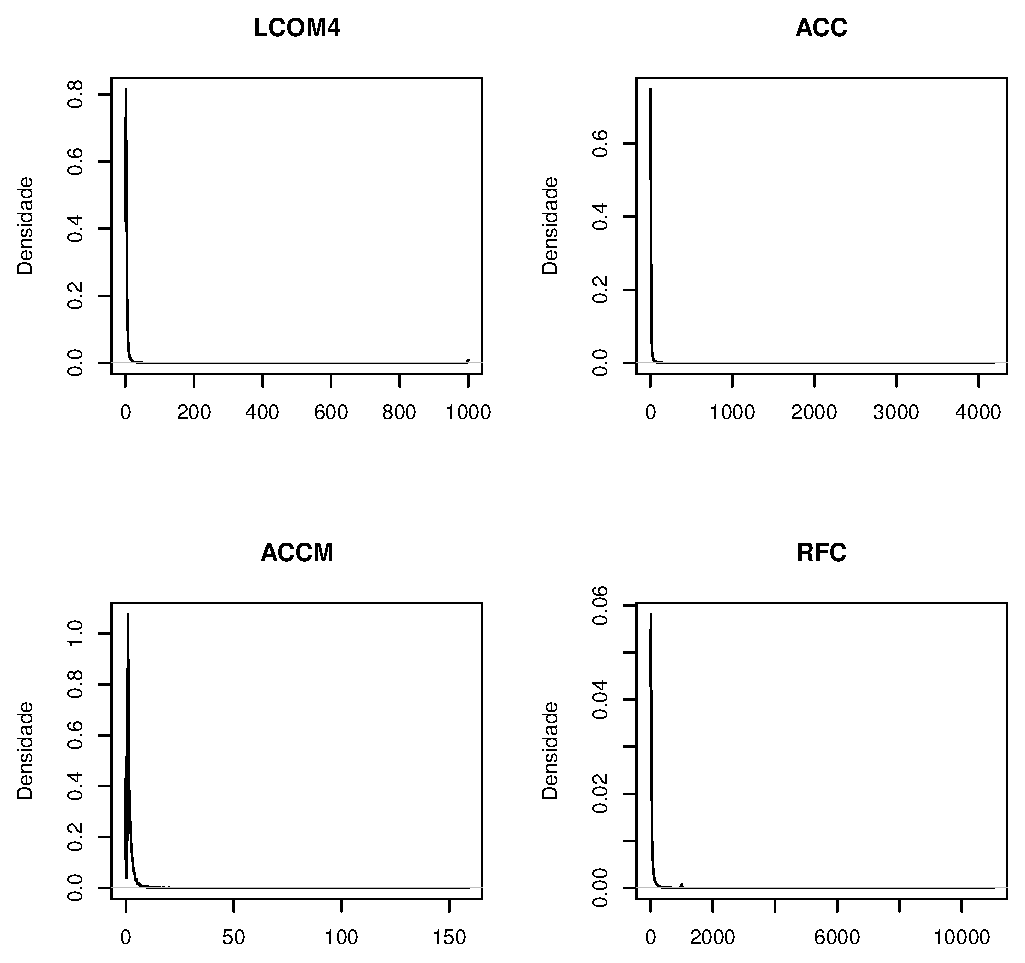
\includegraphics [keepaspectratio=true,scale=0.70]{figuras/android510dist.eps}
\caption{Distribuição de valores para as métricas LCOM4, ACC, ACCM e RFC}
\label{fig:android510dist}
\end{figure}

Com os dados coletados e devidamente preparados, várias conclusões podem ser tiradas dos valores das métricas e sua evolução ao longo do tempo. Esta seção é focada na análise subjetiva dos dados, tentando explicar seu comportamento com relação às características do sistema, compará-los a outros estudos, e até mesmo comparar com dados de métricas em aplicativos, utilizando os próprios aplicativos do sistema como base de comparação.


\subsection{Distribuição dos dados}

Os gráficos na Figura~\ref{fig:android510dist} apresentam as distribuições dos dados para as métricas LCOM4, ACC, ACCM e RFC. Podemos perceber que em todos os casos a densidade de probabilidade apresenta uma distribuição de cauda longa, já demonstrando que a média desses valores não é igual a mediana, e não é significativa. 

Nas tabelas que serão discutidas nas seção seguintes, percebe-se que a mediana, no percentil 50, não representa de forma alguma os dados como faria numa distribuição normal. Para muitas métricas esse percentil apresenta nada mais que o ideal teórico que na prática não é comum, como nas métricas ACCM, NOC, LCOM4 e ACC. Assim, serão utilizados percentis 75, 90 e 95 para análise cada métrica, assim como feito por \citeonline{meirelles2013}. 

\subsection{Average Method Lines Of Code}

\begin{table}[!htb]
\scalefont{.7}
\documentclass[a4paper]{article}
\usepackage[T1]{fontenc}
\usepackage[latin1]{inputenc}
\begin{document}
\begin{tabular}{|l|l|l|l|l|l|l|l|l|l|l|l|}
\hline
version&min&1\%&5\%&10\%&25\%&50\%&75\%&90\%&95\%&99\%&max\\
\hline
android-1.6\_r1.2&0&0&0&0&2.33333333333333&5.57142857142857&11.5&21.5&30&65.8742857142858&312\\
\hline
android-1.6\_r1.5&0&0&0&0&2.33333333333333&5.57142857142857&11.5&21.5&30&65.8742857142858&312\\
\hline
android-2.0\_r1&0&0&0&0&2&5.55555555555556&11.5&21.8461538461538&30.1916666666666&67.8124999999999&390.5\\
\hline
android-2.1\_r2.1p2&0&0&0&0&2&5.625&11.5&21.8571428571429&30.3366666666666&68.4017499999999&395\\
\hline
android-2.2\_r1&0&0&0&0&1.75892857142857&5.8&12.8&26.5&44.2135714285714&156.66&1034\\
\hline
android-2.2.3\_r2&0&0&0&0&1.76587301587301&5.81666666666666&12.8214285714286&26.5&44.1664285714285&156.62&1034\\
\hline
android-2.3\_r1&0&0&0&0&1&5.8&13.6&30.1787878787879&55.3636363636363&164.773333333334&1034\\
\hline
android-2.3.7\_r1&0&0&0&0&1&5.83333333333333&13.7064950980392&30&54.0590277777778&163.397272727272&1034\\
\hline
android-4.0.1\_r1&0&0&0&0&1&5.85714285714286&14&31&54.3731481481482&162.418181818181&1034\\
\hline
android-4.0.4\_r2.1&0&0&0&0&1&5.85714285714286&14&31&53.9791666666667&162&1034\\
\hline
\end{tabular}
\end{document}

\scalefont{.7}
\caption{Percentis para a métrica \textit{Average Method Lines of Code} no Android}
\label{tab:amloc_android}
\end{table}

\begin{figure}[!htb]
\centering
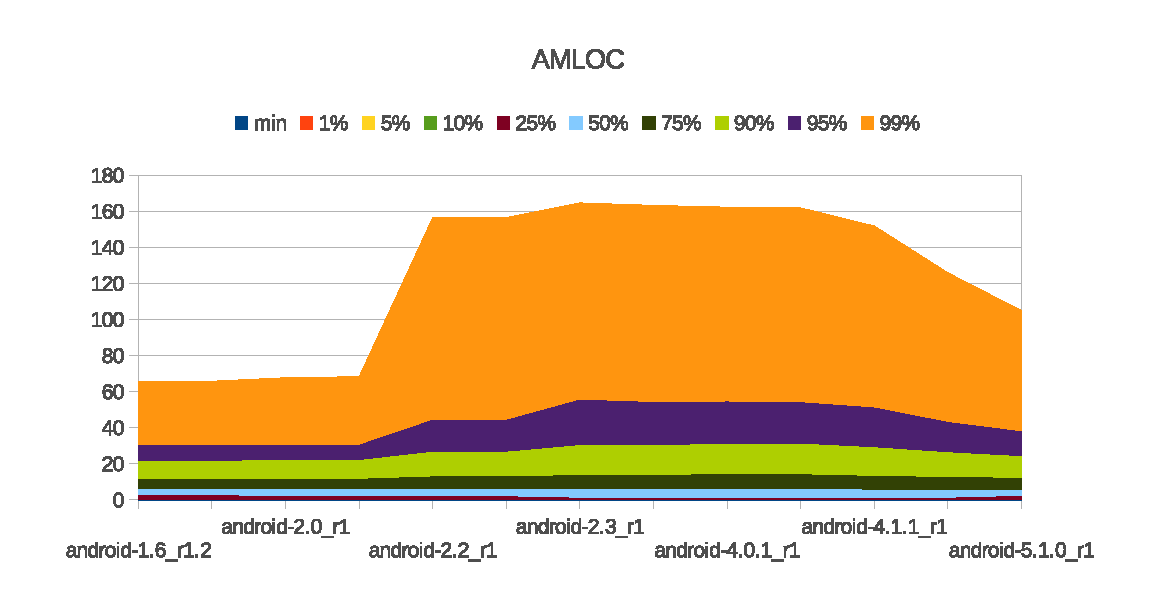
\includegraphics [keepaspectratio=true,scale=0.85]{figuras/graphs/amloc_android.eps}
\caption{Evolução da métrica AMLOC ao longo das versões da API}
\label{fig:amloc_android}
\end{figure}

A Tabela~\ref{tab:amloc_android} apresenta os valores para a métrica AMLOC nas versões do Android analisadas. É facilmente perceptível que a média de linhas de código por método não teve variação relevante. Em todas as versões analisadas, os valores muito frequentes, isto é, percentil 75, são métodos com até 14 linhas de código, enquanto de 14 a 30 aparecem como frequentes, e 31 a 55 pouco frequentes. A Figura~\ref{fig:amloc_android} apresenta a evolução da métrica AMLOC com a API, onde é possível ver uma variação muito pequena de valores para os percentis 75 e 90. O percentil 99 demonstra uma variação maior, mas ele representa dados não frequentes na análise.

Esses são valores que estão de acordo com os apresentados em \citeonline{meirelles2013}, porém levemente menores para os percentis 75 e 90, com aproximadamente 3 linhas de código a menos por método. É possível perceber que os valores se mostraram bem semelhantes para o projeto Android, mesmo considerando o fato que este trabalho estuda apenas a API de desenvolvimento de aplicativos, essencialmente em Java e dentro do diretório ``\textit{frameworks}'' do AOSP, e \citeonline{meirelles2013} analiza todo o código fonte do sistema, que apresenta em sua totalidade uma maior proporção da linguagem C em relação as demais. Esses valores são subsídios para reafirmar que arquivos em C em geral, tem uma maior utilização de linhas de código do que arquivos em Java. \citeonline{oliveira2013} comenta que as diferenças entre as linguagems C/C++/Java para esta métrica não é significativa, uma vez que a sintaxe entre as 3 é bastante semelhante. Dada essa afirmação, podemos comparar os intervalos definidos por ele, chegando a conclusão de que os valores das métricas estão, para todas as versões, abaixo dos valores e regular para os percentis 75 e 90, o que é um bom resultado.

\begin{table}[!htb]
\scalefont{.7}
\begin{tabular}{|l|l|l|l|l|l|l|l|l|l|l|l|l|}
\hline
app&classes&min&1\%&5\%&10\%&25\%&50\%&75\%&90\%&95\%&99\%&max\\
\hline
Launcher2&161&0&0&1&1&3&6.33&10.78&16.9&24.38&48.36&57.5\\
\hline
Settings&722&0&0&0&0&3.63&8&15&21.47&28.5&49.4&80.42\\
\hline
Camera2&462&0&0&0&0&1&4.5&9.85&16.09&21.5&38.28&66.67\\
\hline
Bluetooth&239&0&0&0&2.83&6.02&10.79&22.16&39.86&59.84&111.11&221\\
\hline
QuickSearchBox&196&0&0&1&1&3&4.39&6.17&10.53&13.15&22.28&32\\
\hline
Calculator&10&1&1&1&1&6.67&8.92&13.33&23.26&27.38&30.68&31.5\\
\hline
Terminal&17&0&0.15&0.75&1.85&3.09&8.12&15.29&20.92&29.38&48.27&53\\
\hline
PackageInstaller&19&0&0.68&3.4&4&4.63&6.59&16.98&18.9&22.89&31.45&33.59\\
\hline
Dialer&215&0&0&0&1&3&7&11.13&16.89&19.98&32.02&61.33\\
\hline
Browser&259&0&0&1&1&3.5&6.89&11&19&25.95&46.02&55.33\\
\hline
InCallUI&117&0&0&0&0&1&4.23&12&18.75&23.32&40.77&58\\
\hline
LegacyCamera&214&0&0&0&0.2&4&8.64&15.78&25.47&32.18&69.42&112.67\\
\hline
Gallery2&895&0&0&0&0&3&6&11.5&17.38&21.67&44.36&107\\
\hline
BasicSmsReceiver&5&8.67&8.83&9.47&10.27&12.67&16.33&18.75&18.9&18.95&18.99&19\\
\hline
UnifiedEmail&872&0&0&0&1&3&5&9.71&17&23.67&37.95&139.63\\
\hline
Launcher3&354&0&0&0&0&2.73&5.13&10.59&17.17&24.79&54.71&163.5\\
\hline
Music&75&0&0&0&1&4.1&9.51&16.89&21.76&28.0&48.32&90\\
\hline
Camera&253&0&0&0&1&3&7.42&13&22.37&31.45&72.23&112.67\\
\hline
Email&400&0&0&0&1&3.58&8&15.35&24.49&31.61&63.28&128\\
\hline
Nfc&178&0&0&0&1&3&9.64&18.5&31.63&38&42.48&70.5\\
\hline
Gallery&89&0&0.87&1&1&4&7.63&12.67&19.0&28.6&53.12&55\\
\hline
ContactsCommon&292&0&0&0&1&3.23&7.1&13&19&23.88&34.5&53.33\\
\hline
Contacts&265&0&0&0&1&3&6.45&11.5&18.61&23.72&63.53&86\\
\hline
DeskClock&121&0&0&0&1&5&9.16&15.26&24.02&27.3&30.71&40.13\\
\hline
HTMLViewer&4&5&5.12&5.6&6.2&8&11&14.5&16.6&17.3&17.86&18\\
\hline
Calendar&216&0&0&0&1&5&11.67&19.58&30.95&39.3&90&115.5\\
\hline
Exchange&135&0&0&0&1&4&10.01&17.31&28.41&34.65&44.41&51.25\\
\hline
\end{tabular}

\scalefont{.7}
\caption{Percentis para a métrica \textit{Average Method Lines of Code} nos aplicativos nativos}
\label{tab:amloc_apps}
\end{table}

Os valores apresentados na análise são relativamente baixos quando comparados com outros softwares livres, como demonstrado por \citeonline{meirelles2013}. Da mesma forma, quando olhamos os valores aplicativos do sistema, demonstrados na Tabela~\ref{tab:amloc_apps}, podemos perceber uma grande semelhança nos resultados. Embora alguns poucos aplicativos tenham valores mais elevados para essa métrica, pode-se perceber que os intervalos se mantém válidos para a grande maioria dos aplicativos. Esses valores de aplicativos foram retirados dos aplicativos nativos da ultima versão do sistema analisada (Lollipop 5.1.0), e continuam se mantendo semelhantes ao sistema, como o próprio acoplamento à API sugere.

Os aplicativos do sistema também se mantém dentro dos intervalos bom e regular definidos em \citeonline{oliveira2013}. Os valores para o percentil 95 também se encontram abaixo do valor regular, na maioria dos casos.

Em suma, os valores para os aplicativos se assemelham muito com os valores para as versões da API Android analisadas, levando então a conclusão de que os mesmos intervalos são válidos para as métricas em ambos os casos, embora se possa esperar valores menores em aplicativos, porem com uma maior variância. Essa variância se dá pelo diferente propósito de cada aplicativo, que utiliza pedaços variados do sistema e tem sua codificação adaptada para seu propósito.

Intervalos encontrados:

\begin{itemize}
\item Valores abaixo de 14 se mostraram muito frequentes para os aplicativos e para a API;
\item Enquanto no sistema os valores para o percentil 90 se encontram abaixo de 31, nos aplicativos eles alcançam em poucos casos, ficando em sua maioria abaixo de 25;
\item Valores acima de 31 são pouco frequentes em ambos os casos;
\end{itemize}

\subsection{Average Cyclomatic Complexity per Method}

\begin{figure}[!htb]
\centering
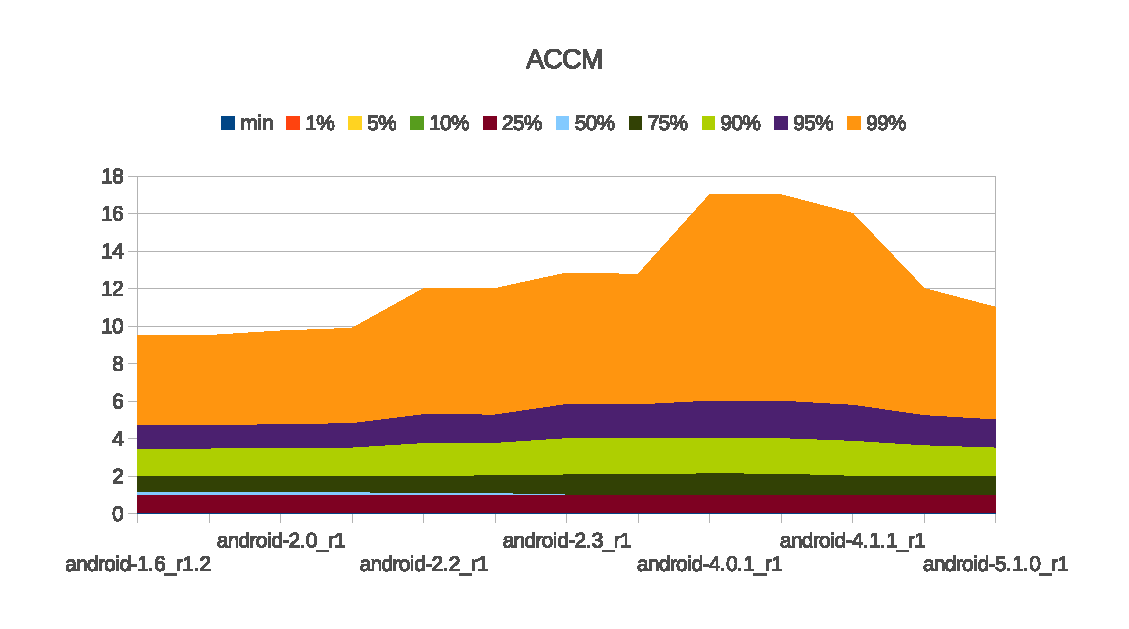
\includegraphics [keepaspectratio=true,scale=0.85]{figuras/graphs/accm_android.eps}
\caption{Evolução da métrica ACCM ao longo das versões da API}
\label{fig:accm_android}
\end{figure}

A Figura~\ref{fig:accm_android} apresenta a evolução de ACCM métrica com a evolução da API. Podemos perceber que essa métrica não teve uma variação grande ao longo das versões nos percentis 75, 90 e 95, e o pouco do valor que ganhou nas versões centrais do gráfico foi sendo novamente reduzido nas versões seguintes.

\begin{table}[!htb]
\scalefont{.7}
\begin{tabular}{|l|l|l|l|l|l|l|l|l|l|l|l|l|}
\hline
versão&classes&min&1\%&5\%&10\%&25\%&50\%&75\%&90\%&95\%&99\%&max\\
\hline
android-1.6\_r1.2&5745&0&0&0&0&1&1.11&2&3.45&4.69&9.5&55\\
\hline
android-1.6\_r1.5&5745&0&0&0&0&1&1.11&2&3.45&4.69&9.5&55\\
\hline
android-2.0\_r1&6331&0&0&0&0&1&1.11&2&3.5&4.75&9.74&59\\
\hline
android-2.1\_r2.1p2&6360&0&0&0&0&1&1.12&2&3.5&4.8&9.88&60\\
\hline
android-2.2\_r1&7352&0&0&0&0&1&1.07&2&3.74&5.28&12&99\\
\hline
android-2.2.3\_r2&7358&0&0&0&0&1&1.07&2.02&3.75&5.26&12&99\\
\hline
android-2.3\_r1&8093&0&0&0&0&1&1&2.07&4&5.82&12.83&99\\
\hline
android-2.3.7\_r1&8240&0&0&0&0&1&1&2.08&4&5.8&12.76&99\\
\hline
android-4.0.1\_r1&11709&0&0&0&0&1&1&2.13&4&6&17&94.33\\
\hline
android-4.0.4\_r2.1&11851&0&0&0&0&1&1&2.11&4&6&17&94.33\\
\hline
android-4.1.1\_r1&14115&0&0&0&0&1&1&2&3.86&5.78&16&99.4\\
\hline
android-4.3.1\_r1&15472&0&0&0&0&1&1&2&3.62&5.23&12&120.4\\
\hline
android-5.1.0\_r1&20129&0&0&0&0&1&1&2&3.5&5&11&158.6\\
\hline
\end{tabular}

\scalefont{.7}
\caption{Percentis para a métrica \textit{Average Cyclomatic Complexity per Method} no Android}
\label{tab:accm_android}
\end{table}

\begin{figure}[!htb]
\centering
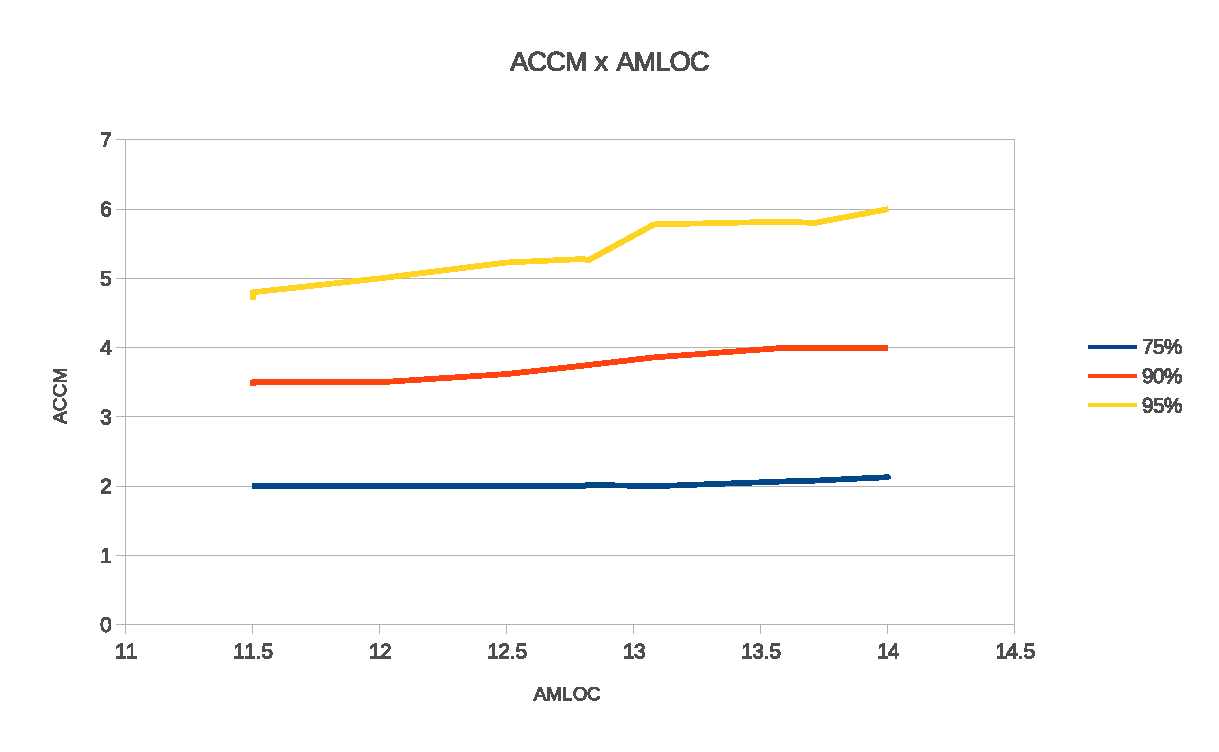
\includegraphics [keepaspectratio=true,scale=0.85]{figuras/ACCMxAMLOC.eps}
\caption{Variação de ACCM por AMLOC para os valores da API apresentados nas Tabelas~\ref{tab:amloc_android} e~\ref{tab:accm_android}}
\label{fig:accmxamloc}
\end{figure}

Uma relação entre ACCM e AMLOC pode ser claramente vista na Tabela~\ref{tab:accm_android} e está melhor demonstrada no gráfico da Figura~\ref{fig:accmxamloc}. Nos valores do percentil 75, que correspondem a valores muito frequentes, as versões de 2.2.3 a 4.0.4 contém os únicos valores para o sistema onde a complexidade ciclomática supera o número 2, e não por acaso são os valores com maior AMLOC nesse percentil como pode ser visto na Tabela~\ref{tab:amloc_android}. Essa relação direta também pode ser vista nos percentis 90 e 95, que representam valores frequentes e pouco requentes, respectivamente.

\begin{table}[!htb]
\scalefont{.7}
\documentclass[a4paper]{article}
\usepackage[T1]{fontenc}
\usepackage[latin1]{inputenc}
\begin{document}
\begin{tabular}{|l|l|l|l|l|l|l|l|l|l|l|l|}
\hline
app&min&1\%&5\%&10\%&25\%&50\%&75\%&90\%&95\%&99\%&max\\
\hline
Launcher2&0&0&1&1&1&1.4&2.09318181818182&3&3.61545454545454&8.67642857142855&11.8666666666667\\
\hline
Settings&0&0&0&0&1&1.57142857142857&2.5&3.66666666666667&4.42857142857143&8&17\\
\hline
Camera2&0&0&0&0&1&1&1.83333333333333&2.66666666666667&3.5&6&8.3\\
\hline
Bluetooth&0&0&0&1&1.33333333333333&2.19337979094077&4&7.95&10.3625&24.2866666666666&49\\
\hline
VoiceDialer&1&1&1&1&1.75&3.5&6.16666666666667&8.52&8.93999999999999&11.388&12\\
\hline
QuickSearchBox&0&0&1&1&1&1.03333333333333&1.66666666666667&2.47142857142857&3&4.67666666666667&5\\
\hline
Calculator&1&1&1&1&1.33333333333333&1.58333333333333&2.66666666666667&3.53333333333333&5.26666666666667&6.65333333333333&7\\
\hline
Mms&0&0&0&0&1&1.28571428571429&2.43650793650793&3.55555555555556&5.4125&10.2285714285714&16\\
\hline
ManagedProvisioning&1&1&1&1&1&2.16764705882353&2.98076923076923&3.24&3.575&5.26000000000001&6\\
\hline
SoundRecorder&1&1.01714285714286&1.08571428571429&1.17142857142857&1.42857142857143&1.6&1.9047619047619&2.94372294372294&3.29004329004329&3.56709956709957&3.63636363636364\\
\hline
Terminal&0&0.15&0.75&1&1&1.5&1.73809523809524&4.8&8.25&10.45&11\\
\hline
PackageInstaller&0&0.17&0.85&1&1&1.2984126984127&2.86458333333333&3.7&4.07058823529412&4.39058823529412&4.47058823529412\\
\hline
SpareParts&1&1.01357142857143&1.06785714285714&1.13571428571429&1.33928571428571&1.67857142857143&2.01785714285715&2.22142857142857&2.28928571428572&2.34357142857143&2.35714285714286\\
\hline
Tag&1&1&1&1&1.1&1.6&1.95833333333334&2.71666666666667&2.975&3.395&3.5\\
\hline
CertInstaller&1&1&1&1&1&1.57142857142857&2.40384615384616&2.7&3.35&3.87&4\\
\hline
KeyChain&0&0.17&0.85&1&1.08333333333333&1.66666666666667&2&2.73&3.51875&3.60375&3.625\\
\hline
Dialer&0&0&0&1&1&1.16666666666667&2&2.77142857142857&3&3.9675&57.8333333333333\\
\hline
Browser&0&0&1&1&1&1.5&2.16666666666667&3.26896551724138&4.03749999999999&7.02500000000001&8.8\\
\hline
PhoneCommon&0&0.17&0.85&1&1&1.16666666666666&1.75&3.51666666666667&5.6125&6.1225&6.25\\
\hline
InCallUI&0&0&0&0&1&1.05555555555555&2.00595238095238&2.76318681318681&4&6.69999999999999&8.33333333333333\\
\hline
CellBroadcastReceiver&1&1&1&1&1.2390350877193&1.76623376623377&3.33928571428572&6.13&9.72&13.636&15\\
\hline
OneTimeInitializer&1&1.02&1.1&1.2&1.5&2&2.5&2.8&2.9&2.98&3\\
\hline
LegacyCamera&0&0&0&0.200000000000003&1&1.6&2.39655172413793&3.36666666666667&4.10599078341013&9.58666666666667&10\\
\hline
Gallery2&0&0&0&0&1&1.375&2.16176470588236&3&3.705&6.01399999999999&11\\
\hline
BasicSmsReceiver&1.33333333333333&1.34333333333333&1.38333333333333&1.43333333333333&1.58333333333334&1.70833333333334&1.99431818181818&2.43409090909091&2.58068181818182&2.69795454545455&2.72727272727273\\
\hline
MusicFX&1&1&1&1&1&2&3.13166666666667&4.96521739130435&7.09782608695653&9.4195652173913&10\\
\hline
TvSettings&0&0&1&1&1&1.40689655172414&2.48026315789474&3.77417582417583&4.7125&6.39749999999998&12\\
\hline
Stk&1&1&1&1.2&2&2.5&3.5&4.724&7.09999999999999&13.82&15.5\\
\hline
UnifiedEmail&0&0&0&1&1&1.16666666666667&1.93541666666667&2.83333333333333&3.66666666666667&6.69166666666666&53\\
\hline
Launcher3&0&0&0&0&1&1.23076923076923&2&3&4&9.87212121212122&30\\
\hline
Music&0&0&0&1&1&1.66666666666667&2.5&3.37436440677966&4.31484517304189&8.96624999999995&18\\
\hline
Camera&0&0&0&1&1&1.49418604651163&2.26559829059829&3.16944801026957&3.96642857142857&9.83000000000001&17\\
\hline
Email&0&0&0&1&1&1.33333333333333&2&3.02222222222222&4.17721139430285&7.50999999999999&19.4\\
\hline
Nfc&0&0&0&1&1&2&3.35294117647059&5.16140350877193&7.86666666666666&9.62&15.5\\
\hline
Gallery&0&0.87&1&1&1&1.6125&2.5&3.35333333333333&3.9125&7.25999999999999&9\\
\hline
ContactsCommon&0&0&0&1&1&1.28571428571429&2&3.44444444444444&4.54166666666667&7&7.5\\
\hline
Contacts&0&0&0&1&1&1.23214285714285&2&3&3.64017857142857&9.74000000000001&21\\
\hline
DeskClock&0&0&0&1&1&1.6875&2.28928571428572&3.25833333333333&3.81&4.48642857142857&5.33333333333333\\
\hline
FMRadio&0&0&0&0&0&0.5&1.69602272727273&2.535&3.27298850574712&9.76500000000001&13.5\\
\hline
\end{tabular}
\newline
\begin{tabular}{|l|l|l|l|l|l|l|l|l|l|l|l|}
\hline
HTMLViewer&1.5&1.51&1.55&1.6&1.75&2&2&2&2&2&2\\
\hline
Calendar&0&0&0&1&1&2&3&4.68&6.325&14.93&19\\
\hline
Exchange&0&0&0&1&1&1.65526315789473&3.2&4.49&5.4112443778111&6.82623913043478&7.66666666666667\\
\hline
\end{tabular}
\end{document}

\scalefont{.7}
\caption{Percentis para a métrica \textit{Average Cyclomatic Complexity per Method} nos aplicativos nativos}
\label{tab:accm_apps}
\end{table}

Essa relação pode ser vista para os aplicativos. Embora não seja totalmente determinístico, no geral aplicativos com maiores valores de AMLOC tendem a ter um maior valor de ACCM, assim como visto na API do sistema. Com exceção do \textit{SMSReceiver}, os 5 aplicativos com maior valor de AMLOC são os que contém maior complexidade do conjunto. 

Reforçando a importância dessa métrica em uma análise estática de código, \citeonline{oliveira2013} define a mesma com um peso adicional em relação a outras métricas em seu estudo. Valores de referencia definidos para esse estudo foram 1 a 3, 3 a 5, e 5 a 7, para excelente, bom e regular, respectivamente. Observando as Tabelas~\ref{tab:accm_android} e~\ref{tab:accm_apps} percebe-se que os valores obtidos neste trabalho estão dentro do intervalo excelente ou bom, para os percentis 75 e 90, e dentro de bom ou regular para o percentil 95, q representa valores menos frequentes. No geral, os resultados indicam que o sistema tem uma boa complexidade ciclomática e que os aplicativos desenvolvidos para o mesmo acompanham essa mesma linha. \citeonline{meirelles2013} definiu intervalos semelhantes para códigos em C, e valores um pouco reduzidos para códigos em C++ e Java (0 a 2, 2 a 4, e 4 a 6 para os percentis 75, 90 e 95 respectivamente).  Os resultados encontrados para a API do sistema Android se encontram todos dentro desses intervalos, confirmando como um bom resultado. Já os aplicativos tem algumas exceções que extrapolam levemente esses valores, mas continuam em sua maioria dentro desses limites.

Baseando-se nessas observações, são considerados os seguintes intervalos:

\begin{itemize}
\item Valores abaixo 2 se mostraram muito frequentes para os aplicativos e para a API, e até 2.5 são considerados excelentes. É importante relembrar que uma complexidade ciclomática 2 implica em afirmar que 2 testes unitários resultam em 100\% de cobertura para esse trecho de código;
\item ACCM menor ou igual a 4 pode ser vista em todas as versões do Android e na grande maioria dos aplicativos dentro do percentil 90, sendo uma referencia para um valor maior mas ainda considerado bom. Os aplicativos do sistema quase não alcançaram esse valor;
\item Valores acima de 4 são considerados regulares e são pouco frequentes em ambos os casos, porém para a API do sistema o percentil 95 chegou a 6. Valores acima de 6 são bem raros e correspondem a uma quantidade estatisticamente desprezível para esta análise;
\end{itemize}

\subsection{Response For a Class}

\begin{table}[!htb]
\scalefont{.7}
\documentclass[a4paper]{article}
\usepackage[T1]{fontenc}
\usepackage[latin1]{inputenc}
\begin{document}
\begin{tabular}{|l|l|l|l|l|l|l|l|l|l|l|l|}
\hline
version&min&1\%&5\%&10\%&25\%&50\%&75\%&90\%&95\%&99\%&max\\
\hline
android-1.6\_r1.2&0&0&0&0&2&10&31&79&133.8&357.480000000003&2858\\
\hline
android-1.6\_r1.5&0&0&0&0&2&10&31&79&133.8&357.480000000003&2858\\
\hline
android-2.0\_r1&0&0&0&0&2&10&31&79&131.5&350&2902\\
\hline
android-2.1\_r2.1p2&0&0&0&0&2&10&32&79&133.049999999999&352.869999999999&2923\\
\hline
android-2.2\_r1&0&0&0&0&2&9&30&77.9000000000005&131.45&372.449999999999&2754\\
\hline
android-2.2.3\_r2&0&0&0&0&2&9&30&78&131.15&372.150000000001&2754\\
\hline
android-2.3\_r1&0&0&0&0&1&8&27&76&129&358&2347\\
\hline
android-2.3.7\_r1&0&0&0&0&1&8&27&76&130&354.219999999999&2347\\
\hline
android-4.0.1\_r1&0&0&0&0&1&7&28&82&140&388&2871\\
\hline
android-4.0.4\_r2.1&0&0&0&0&1&7&28&81&141&391&2921\\
\hline
\end{tabular}
\end{document}

\scalefont{.7}
\caption{Percentis para a métrica \textit{Response For a Class} no Android}
\label{tab:rfc_android}
\end{table}

A API do sistema Android tende a ter um valor relativamente alto de RFC devido a forma como sua arquitetura foi desenhada, como pode ser visto na Tabela~\ref{tab:rfc_android}. Serviços do sistema são acessados muitas vezes através de objetos do sistema, e para seu uso correto alguns métodos devem ser chamados explicitamente. Por exemplo, para acessar o \textit{bluetooth}, não se chama diretamente um método de uma classe \textit{BluetoothAdapter}, pois os serviços do sistema geralmente estão encapsulados e são retornados por um método \textit{get()}, seguidos dos métodos que se deseja utilizar desse serviço. Por exemplo, para verificar dispositivos \textit{bluetooth} próximos, deve-se obter o \textit{adapter} via chamada estática de método para a própria classe para obter a instância, seguida de uma chamada de método para início de \textit{discovery} de dispositivos, e em seguida utilizar os métodos \textit{isDiscoverying()} e \textit{cancelDiscovery()} para controlar a busca. Um acesso direto a uma variável booleana removeria a necessidade da chamada de método \textit{isDiscoverying()}, entretanto perderia seu encapsulamento. De forma geral, encapsulamento de variáveis tende a aumentar o valor de RFC, que conta apenas métodos. 

\begin{figure}[!htb]
\centering
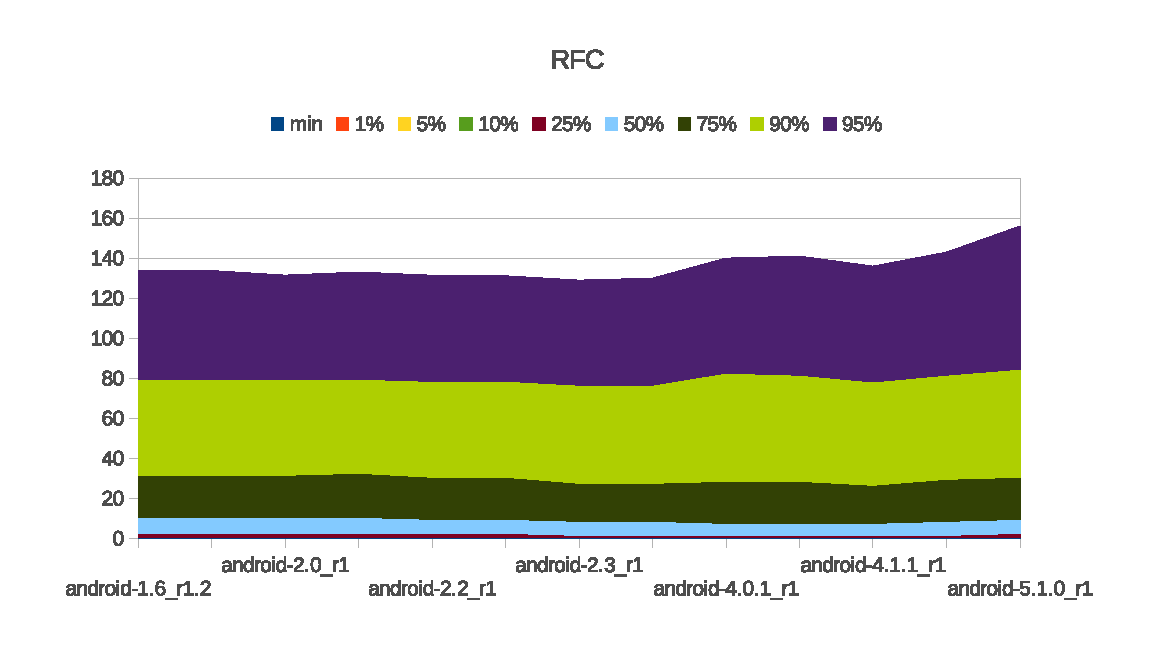
\includegraphics [keepaspectratio=true,scale=0.85]{figuras/graphs/rfc_android.eps}
\caption{Evolução da métrica RFC ao longo das versões da API}
\label{fig:rfc_android}
\end{figure}

Contribuindo para o aumento, o resultado da busca de dispositivos bluetooth é realizado de forma assíncrona na forma de mensagens utilizando \textit{intents} (vide Capítulo~\ref{cap:android-os}), então mais um método é criado dentro de um \textit{receiver} (que pode ser a própria classe estendendo \textit{BroadcastReceiver}) para receber essa mensagem, aumentando um pouco o valor de RFC. Uma comunicação síncrona hipotética com uma chamada estática direta como \textit{BluetoothAdapter.discoverNearDevices()} retornando uma lista seria em teoria uma forma muito mais simples de ser utilizada, porém perderia a proteção do encapsulamento e deixaria de utilizar o comportamento em escopo de objeto para usar em escopo de classe, e também se perderia o maior controle sobre a própria busca que a API dá ao usuário com os métodos adicionais. Além disso, o encapsulamento de serviço dos sistema é um controle adicional que permite que o mesmo escalone melhor a utilização de recursos que necessitem de exclusão mútua. Por exemplo, um acesso direto a câmera dificultaria o sistema de dar acesso a 1 cliente de cada vez, pois afinal, o usuário não consegue usar a câmera, por exemplo, em dois aplicativos simultaneamente.

Comunicações assíncronas são muito usadas ao longo de todo o sistema para utilização de recursos, e então é necessário ter uma forma de receber mensagens de aplicativos e do sistema, o que é feito com a classe \textit{BroadcastReceiver} e implementando métodos específicos da mesma. Mesmo fora do contexto Android, comunicações assíncronas tendem a criar métodos adicionais de comunicação, como é visto no padrão \textit{Observer}, que se assemelha muito a essa comunicação por \textit{Intents}. A Figura~\ref{fig:rfc_android} demonstra que essa métrica não teve variação grande ao longo das versões do Android, tendendo inclusive a um leve aumento nas ultimas versões, demonstrando que os valores altos apresentados são mesmo uma característica da arquitetura do sistema. 

\begin{table}[!htb]
\scalefont{.7}
\begin{tabular}{|l|l|l|l|l|l|l|l|l|l|l|l|}
\hline
app&min&1\%&5\%&10\%&25\%&50\%&75\%&90\%&95\%&99\%&max\\
\hline
Launcher2&0&0&1&1&3.75&12.5&37.25&84.4&178.75&850.719999999999&1061\\
\hline
Settings&0&0&0&0&3&10&31&69&112&229.2&596\\
\hline
Camera2&0&0&0&0&1&6&22&65&113&352.199999999998&752\\
\hline
Bluetooth&0&0&0&2&8&25&68.75&131.3&205.6&468.34&658\\
\hline
VoiceDialer&2&2&2&2&6&14&37&59.4&87.8999999999999&137.58&150\\
\hline
QuickSearchBox&0&0&1&1&3&8&19&30&57.3&115.12&213\\
\hline
Calculator&1&1&1&1&6&8&13&42.8&62.4&78.08&82\\
\hline
Mms&0&0&0&0&2&10&30.5&76.6&122&247.36&788\\
\hline
ManagedProvisioning&1&1&1.85&2&2.25&7.5&49.5&66.4&80.2&93.3&97\\
\hline
SoundRecorder&2&2.84&6.2&10.4&23&28&94&130.6&142.8&152.56&155\\
\hline
Terminal&0&0.15&0.75&1&3&13&47.5&52.5&56.5&64.9&67\\
\hline
PackageInstaller&0&0.17&0.85&2.4&3&10.5&26&62.5000000000001&128&155.2&162\\
\hline
SpareParts&1&1.6&4&7.00000000000001&16&31&46&55&58&60.4&61\\
\hline
Tag&1&1.14&1.7&2.4&4&9&16&20.2&25.5&33.9&36\\
\hline
CertInstaller&1&1&1&1&3.5&6&14.5&86&109.5&128.3&133\\
\hline
KeyChain&0&0.17&0.85&1.7&4&9.5&13.75&21.1&26.3&27.66&28\\
\hline
Dialer&0&0&0&1&3&8.5&25&66.4&113.1&250.74&321\\
\hline
Browser&0&0&1&1&3.25&13&36.75&78.6&124.35&328.89&795\\
\hline
PhoneCommon&0&0.17&0.85&1&3&5.5&9&30.8&43.95&52.79&55\\
\hline
InCallUI&0&0&0&0&1&8&28.25&82.5&120.25&297.349999999999&434\\
\hline
CellBroadcastReceiver&1&1&1&2&5&15.5&26&33.4&54.8&75.63&84\\
\hline
OneTimeInitializer&2&2.18&2.9&3.8&6.5&11&15.5&18.2&19.1&19.82&20\\
\hline
LegacyCamera&0&0&0&0.200000000000003&3&11&38&77.6&139.6&400.76&742\\
\hline
Gallery2&0&0&0&0&3&12&33.75&77.7&110&312.14&595\\
\hline
BasicSmsReceiver&7&7.03&7.15&7.3&7.75&12.5&24.75&38.7&43.35&47.07&48\\
\hline
MusicFX&1&1&1&1.5&2.75&5.5&35.25&125&147.5&194.3&206\\
\hline
TvSettings&0&0&1&1&3&14&41&76.9&107.65&191.599999999999&775\\
\hline
Stk&1&1.16&1.8&2.6&6&18&45&125.6&179.2&304.64&336\\
\hline
UnifiedEmail&0&0&0&1&3&9&25&59&114.5&356.8&1012\\
\hline
Launcher3&0&0&0&0&2&9&31&77.8&144.6&515.640000000001&1407\\
\hline
Music&0&0&0&1&2&6.5&19.75&45.6000000000001&94.9999999999999&155.5&192\\
\hline
Camera&0&0&0&1&2&10&33&80&128.5&307.27&921\\
\hline
Email&0&0&0&1&2.5&9&28&60&93.1999999999999&192.22&399\\
\hline
Nfc&0&0&0&1&3&16&37&93.8&155&263.44&306\\
\hline
Gallery&0&0.87&1&1&4&17&31.5&68.3&118.7&224.66&296\\
\hline
ContactsCommon&0&0&0&1&3&9&22&60&105.5&199.4&271\\
\hline
Contacts&0&0&0&1&3&8.5&23&59&96.25&253.46&463\\
\hline
DeskClock&0&0&0&1&4.75&21&50.25&121.3&151.35&230.25&691\\
\hline
FMRadio&0&0&0&0&0&0.5&18.25&75.4&105.85&277.05&414\\
\hline
\end{tabular}
\newline
\begin{tabular}{|l|l|l|l|l|l|l|l|l|l|l|l|}
\hline
HTMLViewer&1&1.06&1.3&1.6&2.5&4&4.5&4.8&4.9&4.98&5\\
\hline
Calendar&0&0&0&1&4&13&37.5&109.6&160&422.799999999998&1291\\
\hline
Exchange&0&0&0&1&4&14&37.75&72.1&107.55&162.05&224\\
\hline
\end{tabular}

\scalefont{.7}
\caption{Percentis para a métrica \textit{Response For a Class} nos aplicativos nativos}
\label{tab:rfc_apps}
\end{table}


Em suma, na API do sistema, o valor de RFC pode ser considerado alto, porém justificável. Inclusive, o acoplamento entre a própria API de desenvolvimento e o aplicativos faz com que o valor dessa métrica seja alto também para aplicativos desenvolvidos para o Android. E importante lembrar que componentes do sistema se comunicam da mesma forma com outros componentes do sistema como se comunicam com aplicativos desenvolvidos para o mesmo. A Tabela~\ref{tab:rfc_apps} demonstra os valores de RFC para aplicativos nativos.

\citeonline{meirelles2013} define como bons intervalos para projetos Java valores de 0 a 9, 10 a 26, e 27 a 59, para os percentis 75, 90 e 95, respectivamente. Pode-ses perceber que os valores na análise da API obtidos neste trabalho estão bem acima desse valor, estando em seu percentil 75 um valor perto de 30, que seria no máximo regular nessa escala.

Baseando-se em todas essas observações, são considerados os seguintes intervalos:

%TODO rever intervalos
\begin{itemize}
\item Valores abaixo 31 se mostraram muito frequentes para API Android. Para os aplicativos do sistema, existe uma grande variância de valores, porém estando em sua grande maioria abaixo de 38 para o percentil 75.
\item RFC chegou a 130 em aplicativos nativos, porém no geral não alcançam o valor 85. Esse mesmo valor é o limite para a API do sistema.
\item Valores acima de 85 são valores considerados muito altos para a métrica RFC, e são pouco frequentes nos dados analisados.
\end{itemize}

Um intervalo de valores até 38 pode ser considerado bom para aplicativos, e regular no intervalo desse valor até o 85. Acima disso são considerados valores altos. Esses intervalos aqui encontrados estão mais próximos dos limites definidos por \citeonline{meirelles2013} para a Linguagem C do que para Java. Inclusive os valores aqui encontrados aqui para a API Android, essencialmente em Java, se mostram bastante semelhantes aos valores para o projeto Android como um todo, com predominância da linguagem C, encontrados por \citeonline{meirelles2013}. Essa semelhança pode levar a interpretação de que estilos semelhantes de estruturação e design são utilizados em todo o AOSP, independente da linguagem utilizada em cada módulo.

\subsection{Depth of Inheritance Tree / Number of Children}

\begin{figure}[!htb]
\centering
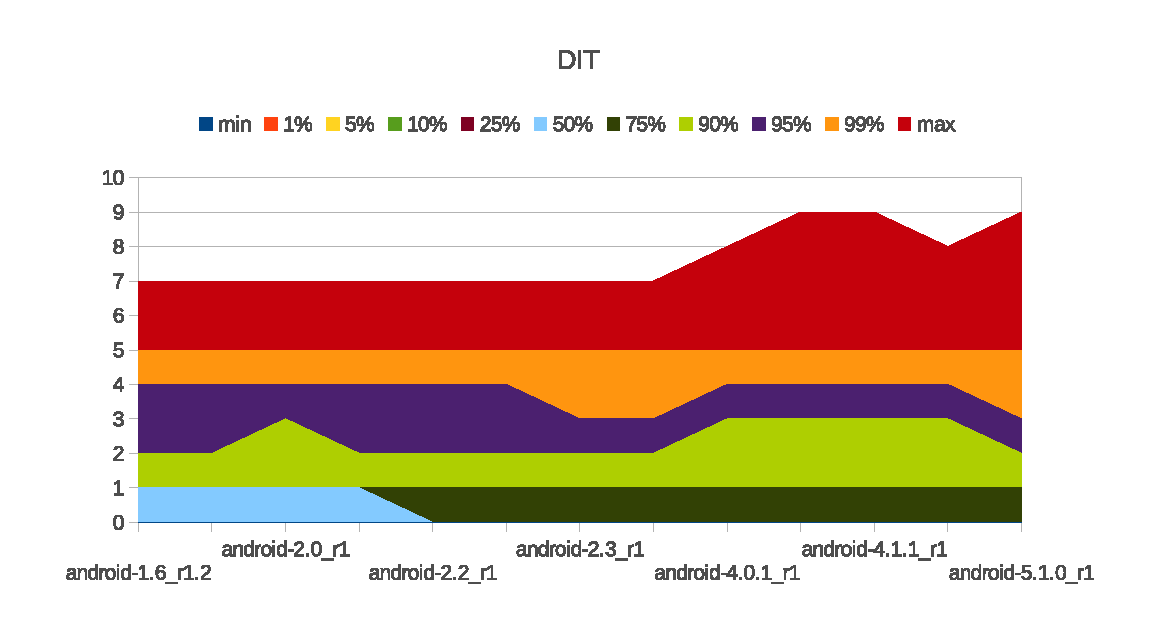
\includegraphics [keepaspectratio=true,scale=0.85]{figuras/graphs/dit_android.eps}
\caption{Evolução da métrica DIT ao longo das versões da API}
\label{fig:dit_android}
\end{figure}

\begin{figure}[!htb]
\centering
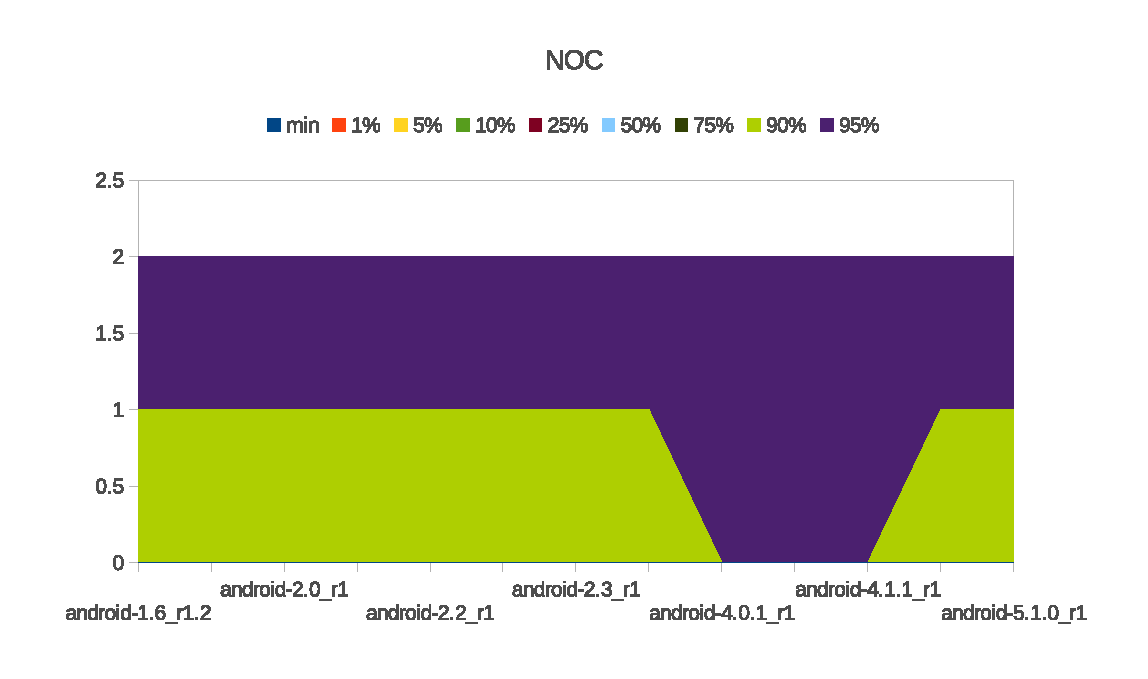
\includegraphics [keepaspectratio=true,scale=0.85]{figuras/graphs/noc_android.eps}
\caption{Evolução da métrica NOC ao longo das versões da API}
\label{fig:noc_android}
\end{figure}

As Figuras~\ref{fig:dit_android} e~\ref{fig:noc_android} demonstram o comportamento dessas métricas com a evolução do sistema. É possível perceber que são valores relativamente baixos e com variação muito pequena para as duas métricas. Para DIT podemos perceber que os valores para cada percentil varia em no máximo 1 em algumas versões e depois voltam ao valor anterior. NOC também se mantém 0 ou 1 para o percentil 90 em todas as versões.

\begin{table}[!htb]
\scalefont{.7}
\begin{tabular}{|l|l|l|l|l|l|l|l|l|l|l|l|l|}
\hline
version&classes&min&1\%&5\%&10\%&25\%&50\%&75\%&90\%&95\%&99\%&max\\
\hline
android-1.6\_r1.2&5745&0&0&0&0&0&1&1&2&4&5&7\\
\hline
android-1.6\_r1.5&5745&0&0&0&0&0&1&1&2&4&5&7\\
\hline
android-2.0\_r1&6331&0&0&0&0&0&1&1&3&4&5&7\\
\hline
android-2.1\_r2.1p2&6360&0&0&0&0&0&1&1&2&4&5&7\\
\hline
android-2.2\_r1&7352&0&0&0&0&0&0&1&2&4&5&7\\
\hline
android-2.2.3\_r2&7358&0&0&0&0&0&0&1&2&4&5&7\\
\hline
android-2.3\_r1&8093&0&0&0&0&0&0&1&2&3&5&7\\
\hline
android-2.3.7\_r1&8240&0&0&0&0&0&0&1&2&3&5&7\\
\hline
android-4.0.1\_r1&11709&0&0&0&0&0&0&1&3&4&5&8\\
\hline
android-4.0.4\_r2.1&11851&0&0&0&0&0&0&1&3&4&5&9\\
\hline
android-4.1.1\_r1&14115&0&0&0&0&0&0&1&3&4&5&9\\
\hline
android-4.3.1\_r1&15472&0&0&0&0&0&0&1&3&4&5&8\\
\hline
android-5.1.0\_r1&20129&0&0&0&0&0&0&1&2&3&5&9\\
\hline
\end{tabular}

\scalefont{.7}
\caption{Percentis para a métrica \textit{Depth of Inheritance Tree} no Android}
\label{tab:dit_android}
\end{table}

\begin{table}[!htb]
\scalefont{.7}
\begin{tabular}{|l|l|l|l|l|l|l|l|l|l|l|l|}
\hline
app&min&1\%&5\%&10\%&25\%&50\%&75\%&90\%&95\%&99\%&max\\
\hline
Launcher2&0&0&0&0&0&1&1&1&2&2.41&3\\
\hline
Settings&0&0&0&0&0&1&2&2&2&3&4\\
\hline
Camera2&0&0&0&0&0&0&1&1&2&3&3\\
\hline
Bluetooth&0&0&0&0&0&0&1&1&2&2&2\\
\hline
VoiceDialer&0&0&0&0&0&0&1&1&1&1&1\\
\hline
QuickSearchBox&0&0&0&0&0&1&1&2&3&5&5\\
\hline
Calculator&0&0&0&0&0&1&1&1&1&1&1\\
\hline
Mms&0&0&0&0&0&1&1&2&3&4&6\\
\hline
ManagedProvisioning&0&0&0&0&0&0&1&1&1&1&1\\
\hline
SoundRecorder&0&0&0&0&0&1&1&1&1&1&1\\
\hline
Terminal&0&0&0&0&0&0&1&1&1&1&1\\
\hline
PackageInstaller&0&0&0&0&0&1&1&1&1&1&1\\
\hline
SpareParts&1&1&1&1&1&1&1&1&1&1&1\\
\hline
Tag&0&0&0&0&0&1&1&1&1&1&1\\
\hline
CertInstaller&0&0&0&0&0.5&1&1.5&2&2&2&2\\
\hline
KeyChain&0&0.17&0.85&1&1&1&1&1&1&1&1\\
\hline
Dialer&0&0&0&0&0&0.5&1&1&1&2&2\\
\hline
Browser&0&0&0&0&0&1&1&1&2&2&2\\
\hline
PhoneCommon&0&0&0&0&0&0&1&1&1.15&1.83&2\\
\hline
InCallUI&0&0&0&0&0&0&1&1&2&2&2\\
\hline
CellBroadcastReceiver&0&0&0&0&1&1&1&1&1.45&2&2\\
\hline
OneTimeInitializer&1&1&1&1&1&1&1&1&1&1&1\\
\hline
LegacyCamera&0&0&0&0&0&0&1&2&2&3&4\\
\hline
Gallery2&0&0&0&0&0&1&1&2&2&3&4\\
\hline
BasicSmsReceiver&1&1&1&1&1&1&1&1&1&1&1\\
\hline
MusicFX&0&0&0&0&0&1&1&1.5&2.25&2.85&3\\
\hline
TvSettings&0&0&0&0&0&1&1&2&3&4&4\\
\hline
Stk&0&0&0&0&1&1&1&1&1&1&1\\
\hline
UnifiedEmail&0&0&0&0&0&1&1&2&2&3&4\\
\hline
Launcher3&0&0&0&0&0&1&1&1&2&3&3\\
\hline
Music&0&0&0&0&0&1&1&1&1&1&1\\
\hline
Camera&0&0&0&0&0&0&1&1&2&3&3\\
\hline
Email&0&0&0&0&0&1&1&1&2&2&3\\
\hline
Nfc&0&0&0&0&0&0&1&1&1&1&1\\
\hline
Gallery&0&0&0&0&0&1&1&2&2&3&3\\
\hline
ContactsCommon&0&0&0&0&0&1&1&1&2&3.10000000000002&5\\
\hline
Contacts&0&0&0&0&0&1&1&1&2&2&3\\
\hline
DeskClock&0&0&0&0&0&1&1&2&2&3&3\\
\hline
FMRadio&0&0&0&0&0&0&1&1&1&1&1\\
\hline
\end{tabular}
\newline
\begin{tabular}{|l|l|l|l|l|l|l|l|l|l|l|l|}
\hline
HTMLViewer&1&1&1&1&1&1&1&1&1&1&1\\
\hline
Calendar&0&0&0&0&0&1&1&1&2&2&2\\
\hline
Exchange&0&0&0&0&0&1&1&1&2&2&2\\
\hline
\end{tabular}

\scalefont{.7}
\caption{Percentis para a métrica \textit{Depth of Inheritance Tree} nos aplicativos nativos}
\label{tab:dit_apps}
\end{table}

A primeira observação sobre o dados das Tabela~\ref{tab:dit_android} e~\ref{tab:dit_apps} é que elas contém um número grande de zeros até o percentil 50. Como a linguagem Java representa mais de 85\% da amostra, vários desses zeros estão presentes também na linguagem Java. O que tiramos disso é que a ferramenta Analizo não contabiliza a classe Object na métrica DIT, pois caso contabilizasse o valor mínimo para o Java seria 1, visto que todo objeto Java herda de Object. Tirando esse fato não temos muitas surpresas, os valores são em geral baixos, chegando a no máximo 4 até o percentil 95 em todos as versões da API, demonstrando valores bem menores dos que os intervalos definidos por \citeonline{meirelles2013} para Java, que chegam até 2, 4 e 6 para os percentis 75, 90 e 95, respectivamente. \citeonline{oliveira2013} utiliza os mesmos intervalos para excelente, bom, e regular, respectivamente. \citeonline{ferreira2009} não define intervalos para essa métrica, mas indica um valor 2 como referência.

\begin{table}[!htb]
\scalefont{.7}
\begin{tabular}{|l|l|l|l|l|l|l|l|l|l|l|l|l|}
\hline
version&classes&min&1\%&5\%&10\%&25\%&50\%&75\%&90\%&95\%&99\%&max\\
\hline
android-1.6\_r1.2&5745&0&0&0&0&0&0&0&1&2&7&110\\
\hline
android-1.6\_r1.5&5745&0&0&0&0&0&0&0&1&2&7&110\\
\hline
android-2.0\_r1&6331&0&0&0&0&0&0&0&1&2&7&122\\
\hline
android-2.1\_r2.1p2&6360&0&0&0&0&0&0&0&1&2&7&124\\
\hline
android-2.2\_r1&7352&0&0&0&0&0&0&0&1&2&6&141\\
\hline
android-2.2.3\_r2&7358&0&0&0&0&0&0&0&1&2&6&141\\
\hline
android-2.3\_r1&8093&0&0&0&0&0&0&0&1&2&6&147\\
\hline
android-2.3.7\_r1&8240&0&0&0&0&0&0&0&1&2&6&149\\
\hline
android-4.0.1\_r1&11709&0&0&0&0&0&0&0&0&2&6&261\\
\hline
android-4.0.4\_r2.1&11851&0&0&0&0&0&0&0&0&2&6&262\\
\hline
android-4.1.1\_r1&14115&0&0&0&0&0&0&0&0&2&6&295\\
\hline
android-5.1.0\_r1&20129&0&0&0&0&0&0&0&1&2&6&398\\
\hline
\end{tabular}

\scalefont{.7}
\caption{Percentis para a métrica \textit{Number of Children} no Android}
\label{tab:noc_android}
\end{table}

A API do sistema se manteve dentro dos intervalos excelente ou bom definidos nesses outros trabalhos citados em todos os percentis analisados nesse trabalho. Os aplicativos se mantiveram dentro do intervalo excelente em todos os percentis, não ultrapassando o valor 2. Em geral, projetos mais simples tendem a fazer menos reúso de código fonte por meio de herança. Oportunidades para uma boa utilização desse recurso de orientação a objetos aparecem com o crescimento do projeto. Dessa forma, é esperado que aplicativos realmente tenham valores menores de DIT e NOC.

A Tabela~\ref{tab:noc_android} apresenta os valores da métrica NOC para o sistema Android. Percebe-se que a maioria das classes não tem filhos, tendo 0 como valor muito frequente em todas as versões da API do sistema. Da mesma forma que a métrica DIT, os valores encontrados aqui são relativamente baixos. \citeonline{meirelles2013} define para projetos Java o valor 0 como muito frequente, 1 a 2 frequente e 3 pouco frequente. O que encontramos aqui é 0 muito frequênte, 0 a 1 como frequente, e 2 como pouco frequente.

\begin{table}[!htb]
\scalefont{.7}
\begin{tabular}{|l|l|l|l|l|l|l|l|l|l|l|l|}
\hline
app&min&1\%&5\%&10\%&25\%&50\%&75\%&90\%&95\%&99\%&max\\
\hline
Launcher2&0&0&0&0&0&0&0&1&2&3.41&5\\
\hline
Settings&0&0&0&0&0&0&0&0&1&4&79\\
\hline
Camera2&0&0&0&0&0&0&0&1&2&3.39999999999998&8\\
\hline
Bluetooth&0&0&0&0&0&0&0&0&0&2.63&10\\
\hline
VoiceDialer&0&0&0&0&0&0&0&0.399999999999999&2&2&2\\
\hline
QuickSearchBox&0&0&0&0&0&0&0&2&2&3.06&4\\
\hline
Calculator&0&0&0&0&0&0&0&1&1&1&1\\
\hline
Mms&0&0&0&0&0&0&0&1&2&5&10\\
\hline
ManagedProvisioning&0&0&0&0&0&0&0&0&0.149999999999999&1.63&2\\
\hline
SoundRecorder&0&0&0&0&0&0&0&0.6&0.8&0.96&1\\
\hline
Terminal&0&0&0&0&0&0&0&0&0&0&0\\
\hline
PackageInstaller&0&0&0&0&0&0&0&0&0&0&0\\
\hline
SpareParts&0&0&0&0&0&0&0&0&0&0&0\\
\hline
Tag&0&0&0&0&0&0&0&0&2.09999999999999&6.02&7\\
\hline
CertInstaller&0&0&0&0&0&0&0&0&1.5&2.7&3\\
\hline
KeyChain&0&0&0&0&0&0&0&0&0&0&0\\
\hline
Dialer&0&0&0&0&0&0&0&1&1&2&3\\
\hline
Browser&0&0&0&0&0&0&0&1&2&2.43000000000001&4\\
\hline
PhoneCommon&0&0&0&0&0&0&0&0&0.149999999999999&0.829999999999998&1\\
\hline
InCallUI&0&0&0&0&0&0&0.25&1&2&5.69999999999999&7\\
\hline
CellBroadcastReceiver&0&0&0&0&0&0&0&0&0.449999999999999&1&1\\
\hline
OneTimeInitializer&0&0&0&0&0&0&0&0&0&0&0\\
\hline
LegacyCamera&0&0&0&0&0&0&0&1&2&3&8\\
\hline
Gallery2&0&0&0&0&0&0&0&1&2&8&17\\
\hline
BasicSmsReceiver&0&0&0&0&0&0&0&0&0&0&0\\
\hline
MusicFX&0&0&0&0&0&0&0&1&1&1&1\\
\hline
TvSettings&0&0&0&0&0&0&0&1&3&5.52999999999997&22\\
\hline
Stk&0&0&0&0&0&0&0&0&0&0&0\\
\hline
UnifiedEmail&0&0&0&0&0&0&0&1&2&5&17\\
\hline
Launcher3&0&0&0&0&0&0&0&1&2&3.48000000000002&7\\
\hline
Music&0&0&0&0&0&0&0&0&0&2.69999999999996&10\\
\hline
Camera&0&0&0&0&0&0&0&1&2&3&5\\
\hline
Email&0&0&0&0&0&0&0&1&2&4.05999999999995&9\\
\hline
Nfc&0&0&0&0&0&0&0&0.400000000000006&1&2&2\\
\hline
Gallery&0&0&0&0&0&0&0&1&2&6.38999999999999&9\\
\hline
ContactsCommon&0&0&0&0&0&0&0&0&1&4.30000000000007&15\\
\hline
Contacts&0&0&0&0&0&0&0&1&1&2.37&9\\
\hline
DeskClock&0&0&0&0&0&0&0&1&1&2&5\\
\hline
FMRadio&0&0&0&0&0&0&0&0&0&1&1\\
\hline
\end{tabular}
\newline
\begin{tabular}{|l|l|l|l|l|l|l|l|l|l|l|l|}
\hline
HTMLViewer&0&0&0&0&0&0&0&0&0&0&0\\
\hline
Calendar&0&0&0&0&0&0&0&0&1&4&8\\
\hline
Exchange&0&0&0&0&0&0&0&0&3&8.68999999999991&15\\
\hline
\end{tabular}

\scalefont{.7}
\caption{Percentis para a métrica \textit{Number of Children} nos aplicativos nativos}
\label{tab:noc_apps}
\end{table}

A tabela~\ref{tab:noc_apps} demonstra que os mesmos valores de NOC discutidos para a API do Android são válidos para os aplicativos nativos da plataforma. 

De forma geral, a complexidade da API android com relação a árvore de herança é relativamente baixa, e isso é refletido nos seus aplicativos, que pelo seu tamanho tem complexidade de herança ainda menor. Os valores de DIT e NOC são muito bons tanto para a API do sistema quanto para os aplicativo desenvolvidos para o mesmo. Vale ressaltar que ambas as métricas são calculadas apenas para linguagem OO, sendo que para C o valor é sempre 0. Como C representa cerca de 2\% das amostras, os resultados não são afetados de forma significativa.

Sobre árvore de herança, consideramos os seguintes intervalos para o Android:

\begin{itemize}
\item DIT até 1 e NOC igual a 0 são valores muito frequentes em todas as amostras.
\item DIT até 2 e NOC igual a 1 são valores frequentes em todas as amostras.
\item DIT até 4 e NOC igual a 2 são valores pouco frequentes para a API, mas para seus aplicativos os valores de DIT no percentil 95 permanecem no número 2.
\end{itemize}

\subsection{Lack of Cohesion in Methods}

\begin{figure}[!htb]
\centering
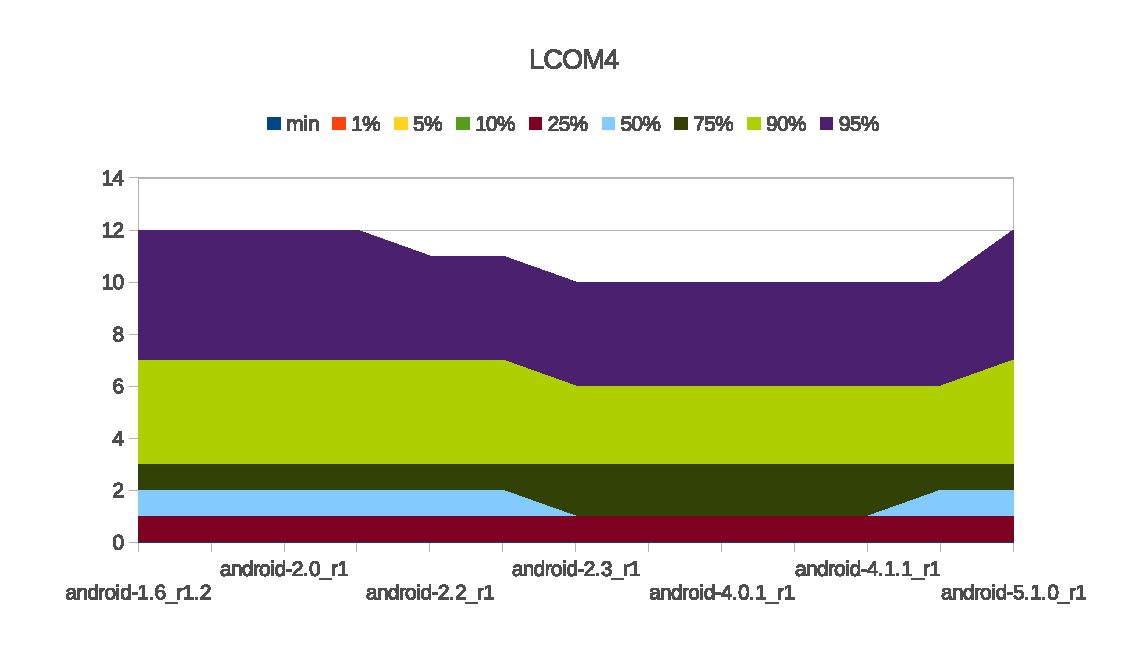
\includegraphics [keepaspectratio=true,scale=0.85]{figuras/graphs/lcom4_android.eps}
\caption{Evolução da métrica LCOM4 ao longo das versões da API}
\label{fig:lcom4_android}
\end{figure}

A Figura~\ref{fig:lcom4_android} apresenta a continuidade dos valores para LCOM na API do android, que, mesmo quado variam de uma versão para outra, retornam aos valores antigos, circulando acerca de um pequeno range de valores. Para o percentil 75, que representa valores muito frequentes, o gráfico demonstra uma linha reta horizontal em verde escuro que não desviou do valor 3 em nenhuma versão da API.

\begin{table}[!htb]
\scalefont{.7}
\begin{tabular}{|l|l|l|l|l|l|l|l|l|l|l|l|l|}
\hline
version&classes&min&1\%&5\%&10\%&25\%&50\%&75\%&90\%&95\%&99\%&max\\
\hline
android-1.6\_r1.2&5745&0&0&0&0&1&2&3&7&12&33&254\\
\hline
android-1.6\_r1.5&5745&0&0&0&0&1&2&3&7&12&33&254\\
\hline
android-2.0\_r1&6331&0&0&0&0&1&2&3&7&12&32&253\\
\hline
android-2.1\_r2.1p2&6360&0&0&0&0&1&2&3&7&12&33&253\\
\hline
android-2.2\_r1&7352&0&0&0&0&1&2&3&7&11&31&253\\
\hline
android-2.2.3\_r2&7358&0&0&0&0&1&2&3&7&11&31&253\\
\hline
android-2.3\_r1&8093&0&0&0&0&1&1&3&6&10&31&253\\
\hline
android-2.3.7\_r1&8240&0&0&0&0&1&1&3&6&10&31&253\\
\hline
android-4.0.1\_r1&11709&0&0&0&0&1&1&3&6&10&32.9200000000001&253\\
\hline
android-4.0.4\_r2.1&11851&0&0&0&0&1&1&3&6&10&32&253\\
\hline
android-4.1.1\_r1&14115&0&0&0&0&1&1&3&6&10&31&437\\
\hline
android-5.1.0\_r1&20129&0&0&0&0&1&2&3&7&12&89.1600000000035&1000\\
\hline
\end{tabular}

\scalefont{.7}
\caption{Percentis para a métrica \textit{Lack of Cohesion in Methods} no Android}
\label{tab:lcom4_android}
\end{table}

A Tabela~\ref{tab:lcom4_android} demonstra que em todas as versões da API Android o valor muito frequente é 3. De 3 a 7 são valores frequentes, e de 7 a 12 pouco frequentes. Valores acima de 12 não são frequentes no sistema. 

Embora o valor ideal de LCOM4 seja 1, valores maiores que 1 não são totalmente estranhos. Muitas classes são criadas para representar alguma entidade real, e para manter seu valor semântico devem desempenhar alguns papéis distintos ao mesmo tempo. E isso é mais frequentemente visto em projetos que contém muitos dispositivos físicos acessíveis e utilizáveis no sistema. 

Em dispositivos móveis, por exemplo, tarefas de tirar foto e capturar vídeo, que são bem distintas, são reunidas na classe câmera, que representa o dispositivo físico que contempla essas funcionalidades. Essa representação de hardware em uma classe específica auxilia a manter uma maior organização no código, e mesmo que sejam tarefas distintas, resultando possivelmente em um maior valor de LCOM4, as classes ainda podem ser consideradas coesas. Fazer a separação da representação de um dispositivo físico em diversas classes pode não ser tão fácil quanto em um projeto com objetos mais ``abstratos'', que podem ser mais facilmente separados sem prejudicar o entendimento da estrutura do sistema.

\begin{table}[!htb]
\scalefont{.7}
\documentclass[a4paper]{article}
\usepackage[T1]{fontenc}
\usepackage[latin1]{inputenc}
\begin{document}
\begin{tabular}{|l|l|l|l|l|l|l|l|l|l|l|l|}
\hline
app&min&1\%&5\%&10\%&25\%&50\%&75\%&90\%&95\%&99\%&max\\
\hline
Launcher2&0&0&1&1&1&2&4&7.09999999999999&10.1&22.23&42\\
\hline
Settings&0&0&0&0&1&1&3&5&6&10.8&44\\
\hline
Camera2&0&0&0&0&1&1&3&7&11&22&135\\
\hline
Bluetooth&0&0&0&1&1&2&3&8&10.15&21.52&27\\
\hline
VoiceDialer&1&1&1&1&1&1&2&3.2&4&4&4\\
\hline
QuickSearchBox&0&0&1&1&1&2&3&6&13&21.18&30\\
\hline
Calculator&1&1&1&1&1&1&2&5.6&6.8&7.76&8\\
\hline
Mms&0&0&0&0&1&2&3&6.60000000000002&13.9&30.46&41\\
\hline
ManagedProvisioning&1&1&1&1&1&1&2&2&2.15&3.63&4\\
\hline
SoundRecorder&1&1&1&1&1&2&2&2&2&2&2\\
\hline
Terminal&0&0.15&0.75&1&1&1&3&6.5&10.75&17.35&19\\
\hline
PackageInstaller&0&0.17&0.85&1&1&1&3&4.3&5.3&6.66&7\\
\hline
SpareParts&1&1&1&1&1&1&1&1&1&1&1\\
\hline
Tag&1&1&1&1&1&2&3&3.6&4&4&4\\
\hline
CertInstaller&1&1&1&1&1&1&2&2&2&2&2\\
\hline
KeyChain&0&0.17&0.85&1&1&1&2&3.3&4.3&5.66&6\\
\hline
Dialer&0&0&0&1&1&2&3&6&9&15.87&28\\
\hline
Browser&0&0&1&1&1&2&4&6&9&32.8700000000001&54\\
\hline
PhoneCommon&0&0.17&0.85&1&1&1.5&2&3.9&6&6&6\\
\hline
InCallUI&0&0&0&0&1&2&4&6&8&14.95&25\\
\hline
CellBroadcastReceiver&1&1&1&1&1&2&3&3.9&4.45&6.38&7\\
\hline
OneTimeInitializer&1&1.01&1.05&1.1&1.25&1.5&1.75&1.9&1.95&1.99&2\\
\hline
LegacyCamera&0&0&0&0.200000000000003&1&2&3&6&7.39999999999998&22.52&47\\
\hline
Gallery2&0&0&0&0&1&2&3&6&9&17.0699999999999&38\\
\hline
BasicSmsReceiver&1&1&1&1&1&1&1.25&1.7&1.85&1.97&2\\
\hline
MusicFX&1&1&1&1&1&1&3&3.5&4&4&4\\
\hline
TvSettings&0&0&1&1&1&1&2&4&6&7.52999999999997&9\\
\hline
Stk&1&1&1&1&1&1&2&3&3.4&4.68&5\\
\hline
UnifiedEmail&0&0&0&1&1&2&3&6&10.5&25.5999999999999&76\\
\hline
Launcher3&0&0&0&0&1&2&4&7&11&33.8400000000001&51\\
\hline
Music&0&0&0&1&1&2&5&15.7&19.75&45.08&48\\
\hline
Camera&0&0&0&1&1&2&3&6&13&39.8600000000001&65\\
\hline
Email&0&0&0&1&1&2&3&7&13&46.02&144\\
\hline
Nfc&0&0&0&1&1&1&3&9.40000000000001&18&25.48&29\\
\hline
Gallery&0&0.87&1&1&1&1.5&3.25&6&9&17.52&21\\
\hline
ContactsCommon&0&0&0&1&1&2&3&6&7.5&17.1&77\\
\hline
Contacts&0&0&0&1&1&2&4&6&8&15.11&21\\
\hline
DeskClock&0&0&0&1&1&2&3&5&5.05&11.24&24\\
\hline
FMRadio&0&0&0&0&0&0.5&2&6&16.85&35.53&43\\
\hline
\end{tabular}
\newline
\begin{tabular}{|l|l|l|l|l|l|l|l|l|l|l|l|}
\hline
HTMLViewer&1&1&1&1&1&1&1.5&1.8&1.9&1.98&2\\
\hline
Calendar&0&0&0&1&1&2&3&5&6.29999999999998&31.3199999999998&51\\
\hline
Exchange&0&0&0&1&1&2&3&6&12&21.3499999999999&32\\
\hline
\end{tabular}
\end{document}

\scalefont{.7}
\caption{Percentis para a métrica \textit{Lack of Cohesion in Methods} nos aplicativos nativos}
\label{tab:lcom4_apps}
\end{table}

\citeonline{meirelles2013} define para projetos Java intervalos de 0 a 3, 4 a 7, e 8 a 12 para os percentis 75, 90 e 95, respectivamente. Os resultados encontrados aqui acompanharam muito bem esses intervalos.

LCOM4 também contabiliza classes de modelo, e no caso do Java, os \textit{getters} e \textit{setters} acarretam no aumento do valor do resultado da métrica\cite{meirelles2013}. Classes de modelo tem maior representatividade estatística em projetos menores, o que ajuda um pouco a justificar o aumento da métrica para aplicativos do sistema, como pode ser visto na Tabela~\ref{tab:lcom4_apps}. Os intervalos 0 a 4, 4 a 7, e 7 a 12 são válidos para a grande maioria dos aplicativos. Os resultados são muito parecidos com os valores para a API, sendo que a métrica só aumenta em 1 no percentil 75.

\subsection{Afferent Connections per Class}

\begin{table}[!htb]
\scalefont{.7}
\begin{tabular}{|l|l|l|l|l|l|l|l|l|l|l|l|l|}
\hline
version&classes&min&1\%&5\%&10\%&25\%&50\%&75\%&90\%&95\%&99\%&max\\
\hline
android-1.6\_r1.2&5745&0&0&0&0&0&0&3&12&26&137&1820\\
\hline
android-1.6\_r1.5&5745&0&0&0&0&0&0&3&12&26&137&1820\\
\hline
android-2.0\_r1&6331&0&0&0&0&0&0&3&11&25&139&1953\\
\hline
android-2.1\_r2.1p2&6360&0&0&0&0&0&0&3&11&25&139.41&1970\\
\hline
android-2.2\_r1&7352&0&0&0&0&0&0&3&12&25.45&132.98&2027\\
\hline
android-2.2.3\_r2&7358&0&0&0&0&0&0&3&12&26&132.86&2028\\
\hline
android-2.3\_r1&8093&0&0&0&0&0&0&3&11&25&114.08&2052\\
\hline
android-2.3.7\_r1&8240&0&0&0&0&0&0&3&11&25&115.22&2070\\
\hline
android-4.0.1\_r1&11709&0&0&0&0&0&0&3&11&24&122&2681\\
\hline
android-4.0.4\_r2.1&11851&0&0&0&0&0&0&3&11&24&121.5&2711\\
\hline
android-4.1.1\_r1&14115&0&0&0&0&0&0&3&11&24&117.86&2965\\
\hline
android-4.3.1\_r1&15472&0&0&0&0&0&0&3&12&25&121&3789\\
\hline
android-5.1.0\_r1&20129&0&0&0&0&0&0&3&11&22&99.72&4180\\
\hline
\end{tabular}

\scalefont{.7}
\caption{Percentis para a métrica \textit{Afferent Connections per Class} no Android}
\label{tab:acc_android}
\end{table}

\begin{figure}[!htb]
\centering
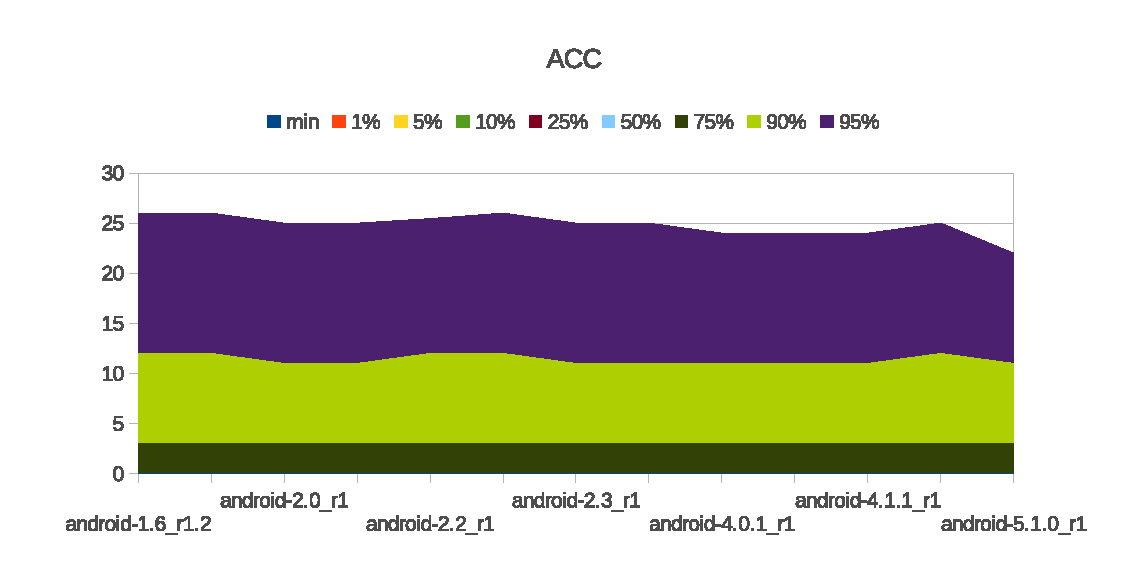
\includegraphics [keepaspectratio=true,scale=0.85]{figuras/graphs/acc_android.eps}
\caption{Evolução da métrica ACC ao longo das versões da API}
\label{fig:acc_android}
\end{figure}

A Figura~\ref{fig:acc_android} e a Tabela~\ref{tab:acc_android} demonstram que os valores da métrica ACC para os percentis 75, 90 e 95 não passam de 3, 12 e 26, respectivamente. \citeonline{oliveira2013} define os intervalos 0 a 2, 2 a 7, e 7 a 15 como excelente, bom e regular para os valores dessa métrica. \citeonline{meirelles2013} define como referencia para java os intervalos 0 a 1, 1 a 5, e 5 a 12 para os percentis 75, 90 e 95, respectivamente.

Os valores encontrados para o Android estão altos quando comparados com esses estudos, e portanto estes não são bem aplicáveis à API do Android, que, como podemos ver na Figura~\ref{fig:acc_android}, contém valores que não parecem ter tendência clara de reduzir para os intervalos considerados bons. A variância dentre as versões da API aqui analisadas é muito baixa, uma vez que quase os mesmos valores podem ser vistos ao longo das versões. Como os intervalos encontrados são constantes ao longo das versões, parecem refletir o design do sistema e podem ser utilizados como referência.

\begin{table}[!htb]
\scalefont{.7}
\begin{tabular}{|l|l|l|l|l|l|l|l|l|l|l|l|l|}
\hline
app&classes&min&1\%&5\%&10\%&25\%&50\%&75\%&90\%&95\%&99\%&max\\
\hline
Launcher2&161&0&0&0&0&0&2&5.25&17.1&26.1&92.38&110\\
\hline
Settings&722&0&0&0&0&0&0&2&6&10&26.6&307\\
\hline
Camera2&462&0&0&0&0&0&0&3&10&18&43.6&122\\
\hline
Bluetooth&239&0&0&0&0&0&1&5&16&31&81.5&169\\
\hline
QuickSearchBox&196&0&0&0&0&0&0&2&6&9&24.56&54\\
\hline
Calculator&10&0&0&0&0&0&2&2&2.4&3.2&3.84&4\\
\hline
Terminal&17&0&0&0&0&0&1&2.25&5&8.25&13.65&15\\
\hline
PackageInstaller&19&0&0&0&0&0&0.5&1&3.3&4.3&5.66&6\\
\hline
Dialer&215&0&0&0&0&0&1&3&6.7&11&16.87&35\\
\hline
Browser&259&0&0&0&0&0&1&3&8&15.15&58.16&122\\
\hline
InCallUI&117&0&0&0&0&0&1&3&6.5&10.5&25.55&93\\
\hline
LegacyCamera&214&0&0&0&0&0&2&6&11.8&16&53.4&91\\
\hline
Gallery2&895&0&0&0&0&0&1&4&11&21.35&75&150\\
\hline
BasicSmsReceiver&5&0&0&0&0&0&0&0.25&0.7&0.85&0.97&1\\
\hline
UnifiedEmail&872&0&0&0&0&0&0&3&10&16&53&160\\
\hline
Launcher3&354&0&0&0&0&0&1&4&14.8&21.8&72.24&124\\
\hline
Music&75&0&0&0&0&0&0&1&2&2.7&6.7&14\\
\hline
Camera&253&0&0&0&0&0&2&5&11.9&18.25&57.13&103\\
\hline
Email&400&0&0&0&0&0&0&1&6&18.1&40.22&201\\
\hline
Nfc&178&0&0&0&0&0&1&4&11.4&18&61.48&67\\
\hline
Gallery&89&0&0&0&0&0&1&4&8.3&13&49.13&50\\
\hline
ContactsCommon&292&0&0&0&0&0&0&1&7&15&69.4&108\\
\hline
Contacts&265&0&0&0&0&0&0&2&5&10&14.37&30\\
\hline
DeskClock&121&0&0&0&0&0&1&6&12&20&32.91&37\\
\hline
HTMLViewer&4&0&0&0&0&0&0&1&1.6&1.8&1.96&2\\
\hline
Calendar&216&0&0&0&0&0&0&4&9&18&29.44&45\\
\hline
Exchange&135&0&0&0&0&0&0&2&5&10.05&71.54&108\\
\hline
\end{tabular}

\scalefont{.7}
\caption{Percentis para a métrica \textit{Afferent Connections per Class} nos aplicativos nativos}
\label{tab:acc_apps}
\end{table}

A Tabela~\ref{tab:acc_apps} demonstra que os valores para os aplicativos do sistema também são maiores que os intervalos definidos em outros estudos. Entretanto, eles são mais parecidos com os valores encontrados dentro da própria API, mais uma vez refletindo a semelhança de aplicativos em relação a mesma, e demonstrando um certo padrão para códigos relacionados ao Android. Para a grande maioria dos aplicativos, os percentis 75, 90 e 95 não ultrapassam os valores 4, 12 e 22, respectivamente.

Consideramos então os seguintes intervalos para o Android:

\begin{itemize}
\item Para o percentil 75, ACC igual a 3 para a API e 4 para aplicativos;
\item 12 é um limite recorrente para o percentil 90 para aplicativos e para a API;
\item Para o percentil 95 em diante, aplicativos tem um valor médio menor que a API, estando com limites até 22 e 26, respectivamente.
\end{itemize}

\subsection{Coupling Factor}

\begin{table}[!htb]
\begin{center}
\scalefont{.7}
\begin{tabular}{|l|l|l|}
\hline
version&classes&cof\\
\hline
android-1.6\_r1.2&5745&0.0013695147\\
\hline
android-1.6\_r1.5&5745&0.001369545\\
\hline
android-2.0\_r1&6331&0.0012379467\\
\hline
android-2.1\_r2.1p2&6360&0.0012384764\\
\hline
android-2.2\_r1&7352&0.0010625123\\
\hline
android-2.2.3\_r2&7358&0.0010616483\\
\hline
android-2.3\_r1&8093&0.0009540904\\
\hline
android-2.3.7\_r1&8240&0.000937113\\
\hline
android-4.0.1\_r1&11709&0.0007400012\\
\hline
android-4.0.4\_r2.1&11851&0.0007300137\\
\hline
android-4.1.1\_r1&14115&0.0005968253\\
\hline
android-4.3.1\_r1&15472&0.0005764279\\
\hline
\end{tabular}

\scalefont{.7}
\caption{Percentis para a métrica \textit{Coupling Factor} no Android}
\label{tab:cof_android}
\end{center}
\end{table}

\begin{figure}[!htb]
\centering
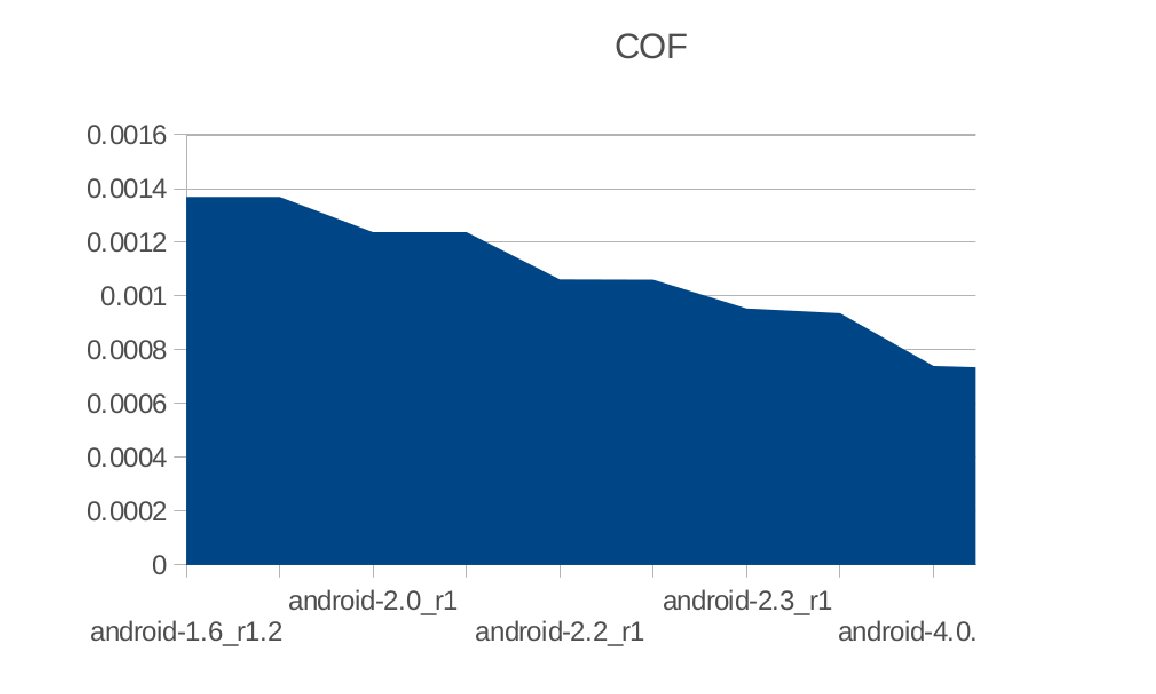
\includegraphics [keepaspectratio=true,scale=0.7]{figuras/graphs/cof_android.eps}
\caption{Evolução da métrica COF ao longo das versões da API}
\label{fig:cof_android}
\end{figure}

%TODO atualizar valores quando obtiver mais versões

O valor de COF para a API do Android ao longo de suas versões caiu de 0.13\% para 0.057\%, como pode ser visto na Figura~\ref{fig:cof_android} e na Tabela~\ref{tab:cof_android}. Isso se dá pelo fato de que, como demonstrado na seção anterior, o valor de ACC permanece relativamente constante enquanto o número de classes aumenta significativamente a cada versão. Essencialmente, o sistema se mostra cada vez mais desacoplado e consequentemente manutenível. 

\begin{table}[!htb]
\begin{center}
\scalefont{.7}
\begin{tabular}{|l|l|l|}
\hline
app&classes&total\_cof\\
\hline
BasicSmsReceiver&5&0.0833333333\\
\hline
Calculator&10&0.1666666667\\
\hline
Calendar&216&0.014844599\\
\hline
Camera&253&0.0195566939\\
\hline
Browser&259&0.0161825476\\
\hline
Bluetooth&239&0.0259014998\\
\hline
ContactsCommon&292&0.0110795118\\
\hline
DeskClock&121&0.0343837535\\
\hline
Dialer&215&0.0119125971\\
\hline
Gallery&89&0.0432340648\\
\hline
Email&400&0.0083122379\\
\hline
Exchange&135&0.0253619122\\
\hline
HTMLViewer&4&0.3333333333\\
\hline
Music&75&0.0111069974\\
\hline
InCallUI&117&0.028035982\\
\hline
Nfc&178&0.0273497689\\
\hline
LegacyCamera&214&0.0230312694\\
\hline
Launcher2&161&0.0415487421\\
\hline
PackageInstaller&19&0.0653594771\\
\hline
QuickSearchBox&196&0.0111551679\\
\hline
Contacts&265&0.0070284595\\
\hline
Camera2&462&0.0079222861\\
\hline
Launcher3&354&0.0148564254\\
\hline
SoundRecorder&6&0.95\\
\hline
Terminal&17&0.1416666667\\
\hline
Settings&722&0.0040414548\\
\hline
Gallery2&895&0.0055753048\\
\hline
UnifiedEmail&872&0.0044023912\\
\hline
\end{tabular}

\scalefont{.7}
\caption{Percentis para a métrica \textit{Coupling Factor} nos aplicativos nativos}
\label{tab:cof_apps}
\end{center}
\end{table}

A Tabela~\ref{tab:cof_apps} apresenta os valores para os aplicativos e nela é possível perceber que o valor de COF não é sempre inversamente proporcional a quantidade de classes como já comentado, embora ele realmente tenha a tendencia a diminuir com o aumento do número de classes. Para os aplicativos, tivemos um range de 33\% para o menor dos projetos, com apenas 4 classes, e 0.4\% para um dos maiores aplicativos.

\citeonline{ferreira2009} apresenta como intervalos os valores de 0 a 0.02 (2\%) como bons , 0.02 a 0.14 (14\%) como regulares, e 0,14 em diante como valores ruins. Podemos perceber que os valores para o sistema Android estão bem abaixo desses valores, sendo considerados então excelentes valores para o fator de acoplamento. Já os aplicativos demonstraram que se mantém nos valores bons quando passam a ter por volta de 200 classes, mas quado muito pequenos se mostraram em sua maioria regulares nessa escala. 

Os intervalos aqui não são considerados em função de seus percentis, mas as seguintes observações podem ser feitas:

\begin{itemize}
\item Espera-se que o valor de COF para o sistema se mostre cada vez menor à medida que novas versões surgem;
\item Aplicativos desenvolvidos para o Android, quando muito pequenos, até poucas dezenas de classes, tendem a ficar abaixo de 10\%, e não devem ultrapassar os 14\% no valor de COF. Valores bem menores ainda podem ser obtidos e são preferíveis;
\item A medida que ganham tamanho de várias dezenas à poucas centenas de classes, os valores de COF para aplicativos não devem ultrapassar os 4\%, entretanto é recomendável que fique abaixo de 2\%. Quando chegam a várias centenas de classes, os valores devem ser menores que 1\%.
\end{itemize}

\subsection{Resumo da discussão}
%TODO trocar nome (esqueci ultima sugestão xD)

\begin{table}[!htb]
\begin{center}
\begin{tabular}{|l|l|l|}
\hline
Métrica & Intervalos                                                                                          & Rótulo                                                                                                                      \\ \hline
AMLOC   & \begin{tabular}[c]{@{}l@{}}{[}0, 14{]}\\ {[}14, 31{]}\\ {[}31, 55{]}\\ {[}55, ...{]}\end{tabular}   & \begin{tabular}[c]{@{}l@{}}Muito Frequente\\ Frequente\\ Pouco Frequente\\ Não Frequente\end{tabular}                       \\ \hline
ACCM    & \begin{tabular}[c]{@{}l@{}}{[}0, 2{]}\\ {[}2, 4{]}\\ {[}4, 6{]}\\ {[}6, ...{]}\end{tabular}         & \begin{tabular}[c]{@{}l@{}}Muito Frequente\\ Frequente\\ Pouco Frequente\\ Não Frequente\end{tabular}                       \\ \hline
RFC     & \begin{tabular}[c]{@{}l@{}}{[}0, 31{]}\\ {[}31, 85{]}\\ {[}85, 140{]}\\ {[}140, ...{]}\end{tabular} & \begin{tabular}[c]{@{}l@{}}Muito Frequente\\ Frequente\\ Pouco Frequente\\ Não Frequente\end{tabular}                       \\ \hline
DIT     & \begin{tabular}[c]{@{}l@{}}{[}0, 1{]}\\ {[}1, 2{]}\\ {[}2, 4{]}\\ {[}4, ...{]}\end{tabular}         & \begin{tabular}[c]{@{}l@{}}Muito Frequente\\ Frequente\\ Pouco Frequente\\ Não Frequente\end{tabular}                       \\ \hline
NOC     & \begin{tabular}[c]{@{}l@{}}0\\ 1\\ 2\\ {[}3, ...{]}\end{tabular}                                    & \begin{tabular}[c]{@{}l@{}}Muito Frequente\\ Frequente\\ Pouco Frequente\\ Não Frequente\end{tabular}                       \\ \hline
LCOM4   & \begin{tabular}[c]{@{}l@{}}{[}0, 3{]}\\ {[}3, 7{]}\\ {[}7, 12{]}\\ {[}12, ...{]}\end{tabular}       & \begin{tabular}[c]{@{}l@{}}Muito Frequente\\ Frequente\\ Pouco Frequente\\ Não Frequente\end{tabular}                       \\ \hline
ACC     & \begin{tabular}[c]{@{}l@{}}{[}0, 3{]}\\ {[}3, 12{]}\\ {[}12, 26{]}\\ {[}26, ...{]}\end{tabular}     & \begin{tabular}[c]{@{}l@{}}Muito Frequente\\ Frequente\\ Pouco Frequente\\ Não Frequente\end{tabular}                       \\ \hline
COF     & \begin{tabular}[c]{@{}l@{}}até 14\%\\ até 4\%\\ até 2\%\end{tabular}                                & \begin{tabular}[c]{@{}l@{}}Para poucas dezenas de classes\\ Para poucas centenas de classes\\ Para várias centenas de classes\end{tabular} \\ \hline
\end{tabular}
\scalefont{.85}
\caption{Intervalos definidos para sistema Android}
\label{tab:final_table_android}
\end{center}
\end{table}

A Tabela~\ref{tab:final_table_android} apresenta um resumo dos intervalos definidos para a API do sistema Android ao longo dessa seção. Embora algumas métricas tenham um indicativo de um problema pontual, como explicado no Capítulo~\ref{cap:metricas} e em outras seções deste capítulo, nenhuma das métricas discutidas neste trabalho deve ser analisada isoladamente.

\subsubsection{Observações acerca das métricas}

Valores baixos de AMLOC são sempre preferíveis, pois métodos mais enxutos tem menor responsabilidade, portanto estão mais sujeitos a reuso, e também são mais fáceis de se ler e se modificar. Entretanto essa métrica é preciso ser analisada em conjunto com outras métricas, como LCOM4 e RFC. Uma classe com muitos métodos privados pequenos tende a ter um valor maior de RFC, o que não implica que esteja mal projetada, desde que os métodos ali presentes estejam bem posicionados segundo o padrão de projeto OO especialista da informação, mantendo por consequência um baixo valor de LCOM4. Como referência geral de resultados para AMLOC, quanto menor o valor, melhor o resultado.

O resultados para a métrica ACCM, que é uma métrica bastante difundida e tem sua aplicabilidade bem clara, relacionados aos AMLOC, dão subsídio para reafirmar que os valores da métrica AMLOC devem ser os menores possíveis para uma boa arquitetura orientada a objetos.

Entender a relação entre ACCM e AMLOC é importante também para pensar em possibilidade de refatoração de um código fonte alvo. Estão claras as consequências de se ter uma alta complexidade ciclomática, mas essa discussão nos leva rapidamente a ter a idéia verificar os métodos da classe e avaliar se seu comportamento está tão enxuto como deveria ser, se algum método não está fazendo mais do que propõe. As vezes dividir o comportamento em tarefas menores possa ser uma solução viável. Dividir o comportamento de um método em 2 provavelmente vai acarretar no aumento da métrica RFC, mas mais uma vez ressalto que o valor de RFC não deve ser analisado por si só. É importante ficar de olho também em métricas como a LCOM quando fazendo esse tipo de refatoração, pois as vezes uma tarefa menor que foi extraída de um método não está coesa na classe onde está e muitas vezes até já esteja implementada em uma outra classe que tem responsabilidade mais congruente com essa tarefa. Remover esse tipo de código duplicado ajuda a reduzir a falta de coesão dentro de uma classe, e todas essas melhorias derivaram do simples fato de perceber uma alta complexidade ciclomática em uma classe.

O ideal em uma classe é obter métodos pequenos com tarefas atômicas e bem definidas, que correspondam às responsabilidades dessa classe. A métrica RFC está diretamente relacionada a Number Of Methods (NOM), uma vez que um aumento neste ultimo implica necessariamente em um aumento em RFC. Uma classe que tenha alto RFC e muitos métodos (valor alto de NOM) pode indicar que está fazendo mais tarefas do que é sua responsabilidade fazer, necessitando talvez rever a sua implementação para aumentar sua coesão. Da mesma forma, um valor alto de RFC e valor baixo de NOM indica que uma classe está fazendo muito o uso de métodos de terceiros, podendo-se inferir que alguns métodos possam ser extraídos para essas classes que estão sendo tanto chamadas, com o objetivo de diminuir o acoplamento entre essas classes.

Alto valor de profundidade de árvore de herança em uma classe pode auxiliar no aumento da métrica RFC, uma vez que todos os comportamentos são herdados. Entretanto não é uma correlação direta significativa entre as duas, visto que a profundidade de herança raramente é alta para o sistema Android, como será discutido nas seções seguintes. Embora valor alto de DIT possa significar maior valor de RFC, valores muito altos de RFC tendem a indicar mais a falta de coesão e alto acoplamento, aumentando assim a complexidade estrutural da classe, e não uma profundidade de herança preocupante.

LCOM4 juntamente com RFC são bons indicadores da organização interna de uma classe, pois ambas as métricas dão subsídios para avaliar coesão. Essencialmente, métricas de coesão e acoplamento estão sempre relacionadas e são as métricas mais indicadas para avaliar a complexidade estrutural de uma classe. A ferramenta Analizo, por exemplo, calcula a métrica Structural Complexity (SC) como produto entre LCOM4 e CBO.

%As Tabelas~\ref{tab:cbo_android} e~\ref{tab:cbo_apps} demonstram que os valores encontrados para CBO na API e nos aplicativos são absurdamente grandes. Não foi encontrado um motivo para tal, podendo então haver algum tipo de problema na ferramenta de captura. O estudo conduzido por \citeonline{meirelles2013} utiliza a mesma ferramenta e não chegou a esses valores aqui encontrados em nenhum projeto, nem mesmo na análise do código fonte completo do sistema Android. Por não conseguirmos identificar exatamente o motivo dessa discrepância de valores, serão consideradas as métricas ACC e COF para acoplamento.

Dentro do escopo de um projeto, pela própria definição da métrica, o valor limite para ACC é o próprio número de classes. Embora o valor seja limitado pelo número de classes, não é possível perceber uma relação direta entre o crescimento do número de classes e o valor de ACC, sendo que essa métrica é mais relacionada à forma como o sistema foi pensado e desenhado do que com o seu tamanho. Entretanto, para análise longitudinal em um mesmo projeto, a relação entre número de classes e COF se mostra válida.

\section{Validação dos intervalos de referência}

Após a obtenção e analise de distribuição dos dados de métricas OO nas diferentes versões do Android e em aplicativos nativos, foram feitos alguns estudos para validar os intervalos de referência definidos na primeira seção deste capítulo. Esses estudos, além de validar os valores definidos previamente de forma subjetiva, também tinham como propósito verificar a possibilidade de utilizar esses dados para auxiliar desenvolvedores no desenvolvimento de aplicativos. 

A partir daí, o passo inicial foi pensar na criação um modelo de regressão que conseguisse predizer o valor ideal de uma métrica OO a partir de uma variável independente de tamanho que representasse a escala do projeto, de forma a obter um valor proporcional daquela métrica. O desenvolvedor então poderia comparar esse valor com o valor real da métrica que o código apresenta, e com os intervalos que foram definidos neste trabalho, e então verificar se mudanças estruturais devem ser feitas.

Após identificadas as limitações e problemáticas com essa abordagem de regressão, o trabalho seguiu um novo caminho em direção à uma comparação mais direta. A ideia vem da proposição de que, julgando a API como um bom exemplo de código, valores próximos aos da API podem ser considerados bons por consequência. 

O passo seguinte foi então avaliar a qualidade um aplicativo a partir da distancia da API no que diz respeito a métricas estáticas de código.

\subsection{Validação por regressão}

A seguir métricas base que foram inicialmente idealizadas para relativização das métricas por regressão polinomial:

\begin{enumerate}
\item Número de classes, realizando uma regressão em escopo de software.
\item Número de classes por pacote, resultando em uma regressão em escopo de ``módulo''.
\item NOM, realizando uma regressão em escopo de classe.
\item AMLOC, realizando uma regressão em escopo de classe.
\end{enumerate}

Não é possível idealizar esse resultado para métricas OO, mensuradas para cada classe, para entradas mais granularizadas como valores de métodos. A grande maioria das métricas tem seus valores para a classe como um todo, não podendo fazer distinção sobre a participação de cada método individualmente dentro daquele valor.

Nenhuma das formas propostas foi realmente implementada, apenas foi realizado uma discussão das possibilidades com as métricas que estavam disponíveis. Métricas de tamanho foram o alvo da regressão como variáveis independentes porque seriam uma forma de abstrair os resultados para projetos de diferentes escalas. Essencialmente os intervalos de valores anteriormente definidos seriam validados se a métrica estivesse de acordo com os mesmos para os parâmetros específicos do projeto sendo analisado, fazendo uma comparação entre o modelo de regressão e a análise manual subjetiva deste trabalho.

\subsubsection{Regressão em escopo de software}

A primeira observação que se faz sobre a realização de regressão em escopo de software utilizando os valores da evolução da API do sistema Android é capacidade de generalização de um modelo. De forma geral, o modelo seria criado com pontos com valores de número de classes variando de 5000 a 20000 classes. Como consequência, argumentamos que o modelo de regressão não teria uma boa capacidade de generalização para projetos muito pequenos, como acontece com aplicativos, que possuem muitas vezes apenas algumas dezenas de classes, e são o alvo principal para utilização dessa regressão. Da mesma forma, a capacidade de predição para projetos que contenham bem mais que 20000 classes também seria prejudicada, uma vez que o modelo de regressão não veria nenhum nesse intervalo. 

\begin{figure}[!htb]
\centering
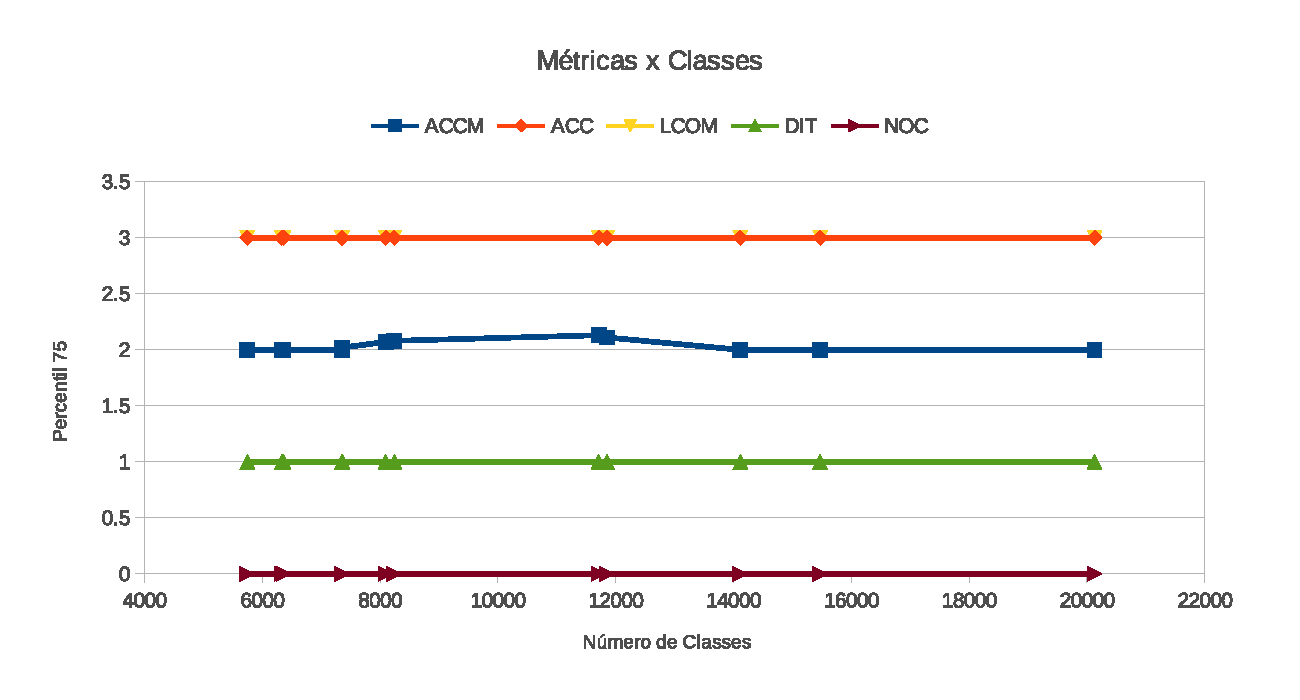
\includegraphics [keepaspectratio=true,scale=0.7]{figuras/metricasxclasses.eps}
\caption{valores dos percentis 75 das métricas DIT, NOC, LCOM, ACC e ACCM em função do número de classes}
\label{fig:metricasxclasses}
\end{figure}

\begin{figure}[!htb]
\centering
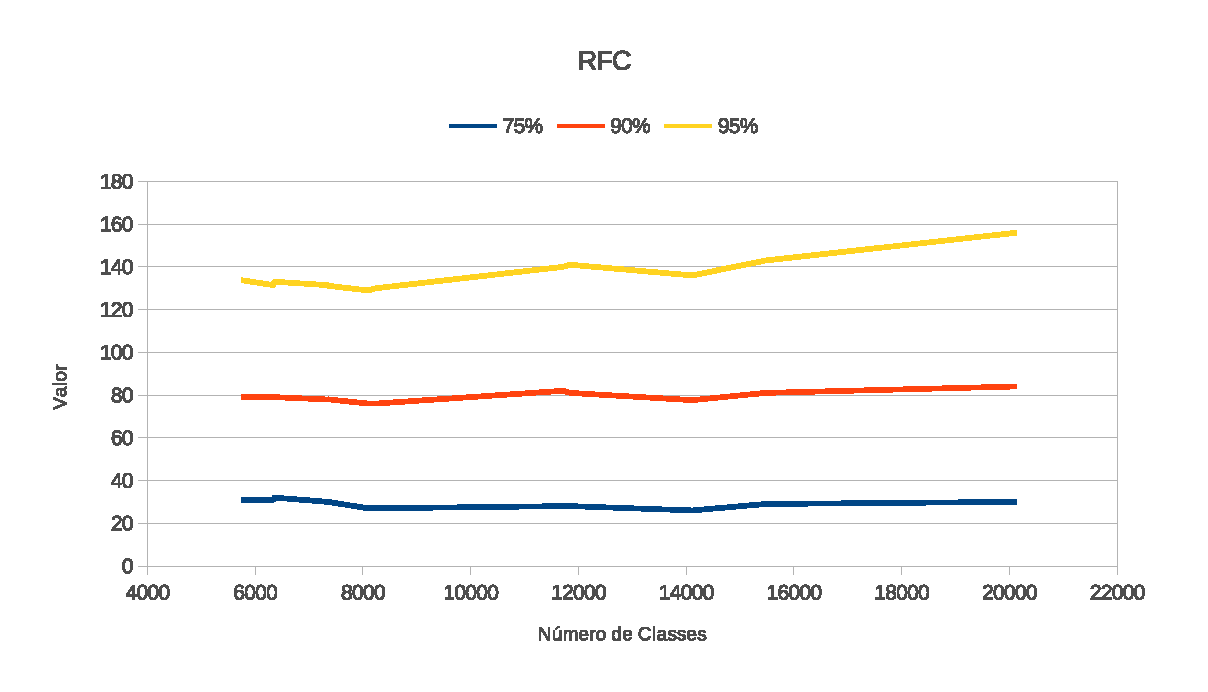
\includegraphics [keepaspectratio=true,scale=0.7]{figuras/rfcxclasses.eps}
\caption{valores dos percentis 75, 90 e 95 de RFC em função do número de classes}
\label{fig:rfcxclasses}
\end{figure}

Para que isso pudesse ser realmente feito, os dados das métricas OO devem ser relacionados com as métricas de tamanho, demonstrando seu valor como dependente do valor dessas métricas. Se os dados obedecem um certo padrão, um funcional pode ser traçado para representar o comportamento dos mesmos. 

Como podemos ver na Figura~\ref{fig:metricasxclasses}, onde é traçado o percentil 75 em função do número de classes, as métricas DIT, NOC, ACC, LCOM4 e ACCM podem ser representadas por uma linha reta horizontal, enquanto RFC, plotada na Figura~\ref{fig:rfcxclasses}, tem dados mais dispersos mas ainda podem ser representados por uma reta horizontal sem perda significativa nos percentis 75 e 90, que correspondem a grande maioria dos dados. Nas tabelas e gráficos apresentados nas seção anterior pode ser confirmado que dentro de cada percentil de cada métrica a variação é pequena. Não foram plotados os valores de outros percentis aqui por diferenciação de escala que exigiria uma quantidade absurda de gráficos, além de não terem tanta importância quanto os valores muito frequêntes apresentados no percentil 75.

Para algumas métricas essa regressão parece ser possível, isto é, um funcional realmente pode ser traçado que representa a variação dos valores das métricas com o número de classes do projeto. Entretanto, para a ínfima variação nos percentis mais significativos para métricas importantes como ACC, LCOM4, DIT, NOC, RFC, ACCM, que são as principais métricas aqui analisadas, argumentamos que um valor referência se mostra tão útil quanto essa regressão, tornando-a desnecessária.

Além de poder utilizar um valor referencia sem perda de valor semântico sobre o valor ideal da métrica, uma regressão em escopo de software da forma como foi proposta, pelo número de classes, não contém, com os dados aqui obtidos, um conjunto suficiente de dados para uma boa regressão. Em suma, temos poucas amostras para realizar esse estudo.

Como um pequeno problema adicional, os dados das métricas para os aplicativos se mostraram levemente diferentes para os dados da API do sistema, mesmo estando bem semelhantes, então argumentamos que utilizar apenas a API do sistema como insumo para o modelo de regressão resultaria em um modelo que não funciona tão bem para predizer valores de métricas de aplicativos. Para os aplicativos, que são projetos distintos, as métricas são extremamente dispersas em relação ao número de classes, tornando difícil representar bem os dados por um polinômio para realizar a regressão. 

Para realização de um modelo de regressão polinomial a nível de software, não foi encontrada ao longo deste trabalho, dadas restrições de tempo e escopo, outra métrica que representasse bem o tamanho do projeto para relativização do resultado das métricas OO. 

\subsubsection{Regressão em escopo de classe}

Como uma segunda tentativa na direção de uma regressão polinomial, foi verificada a possibilidade de utilizar valores das métricas para cada classe, e não para o projeto. Tentamos então avaliar o valor ideal de uma métrica para uma classe, dado alguma variável independente que represente de alguma forma seu tamanho.

\begin{figure}[!htb]
\centering
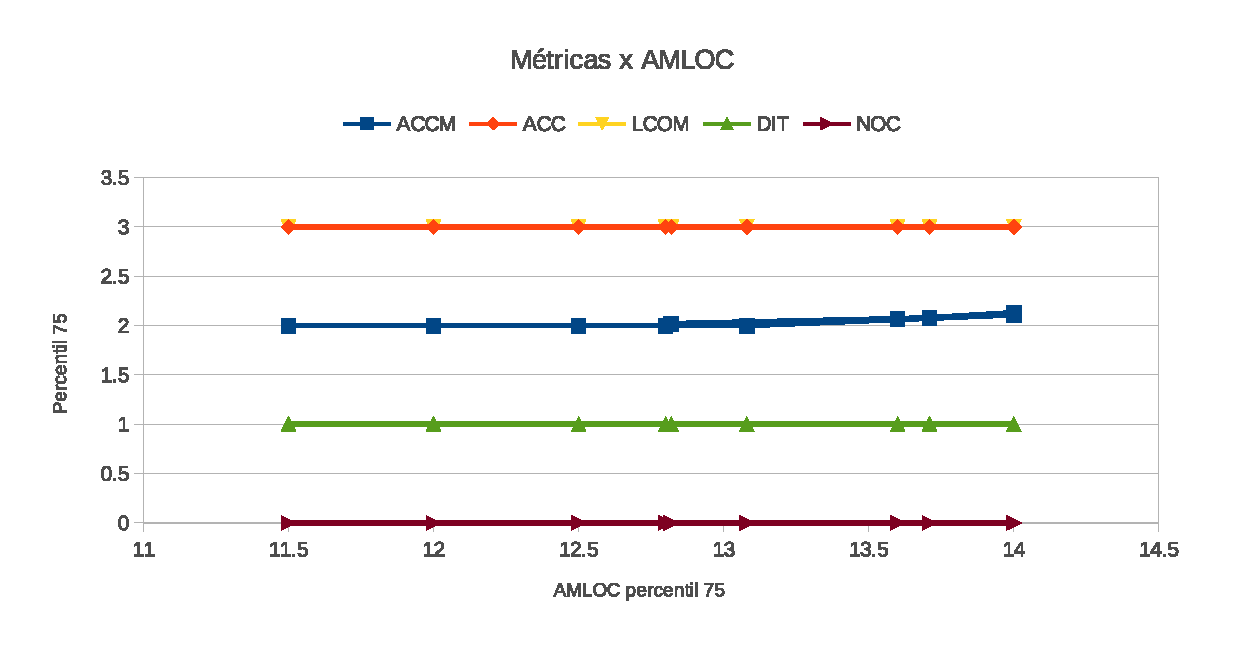
\includegraphics [keepaspectratio=true,scale=0.7]{figuras/metricasxamloc.eps}
\caption{valores dos percentis 75 das métricas DIT, NOC, LCOM, ACC e ACCM em função de AMLOC}
\label{fig:metricasxamloc}
\end{figure}

\begin{figure}[!htb]
\centering
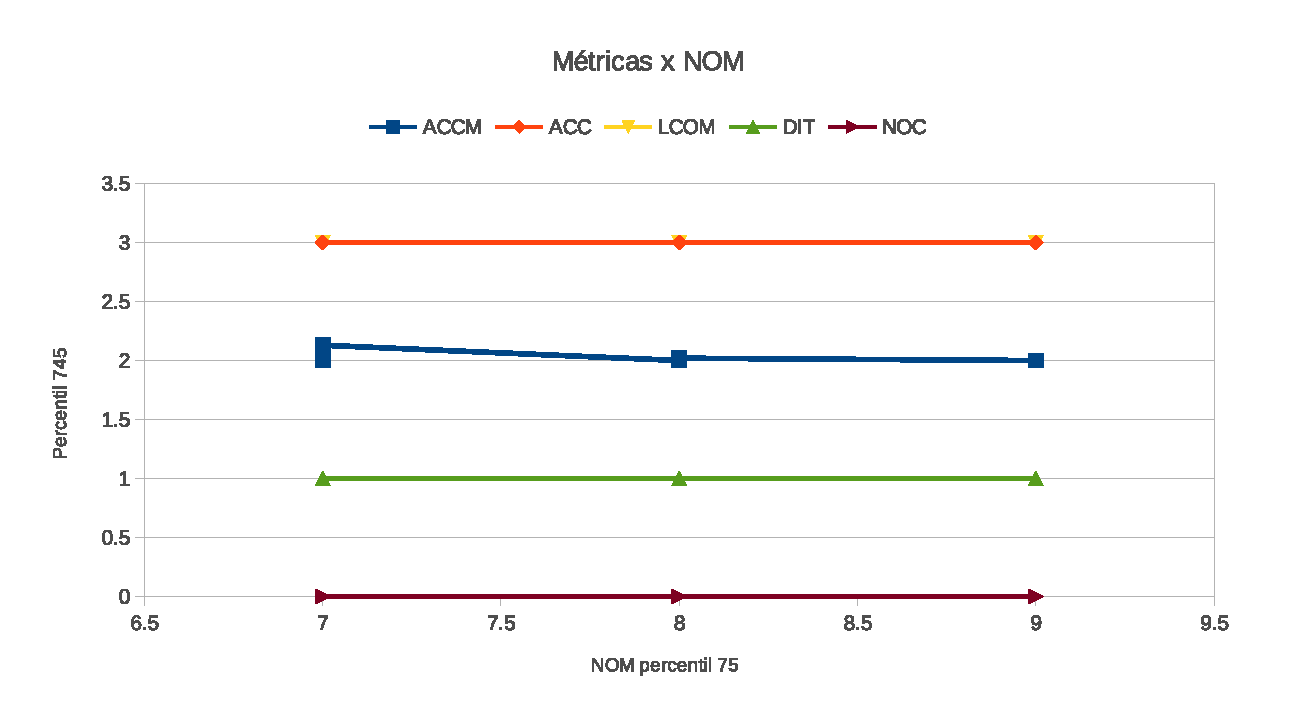
\includegraphics [keepaspectratio=true,scale=0.7]{figuras/metricasxnom.eps}
\caption{valores dos percentis 75 das métricas DIT, NOC, LCOM, ACC e ACCM em função de NOM}
\label{fig:metricasxnom}
\end{figure}

Cada classe dentro de cada versão seria uma amostra para esse método, que teria então um total de mais de 100000 classes. Pensando dessa forma o problema de escala do escopo de software seria resolvido.

O problema nessa abordagem é que as métricas de tamanho que podem ser utilizadas também se mostraram independentes dos valores das métricas OO. Isso faz com que a variação das métricas OO em função de AMLOC ou NOM seja mínima e os dados se apresentem na forma de uma linha horizontal como mostram as Figuras~\ref{fig:metricasxamloc} e~\ref{fig:metricasxnom}. Na verdade, apenas pelo fato de essas métricas não variarem muito ao longo das versões, já se pode prever esse resultado.

Os valores das métricas não são relacionados com os valores dessas métricas de tamanho, como mostra a matriz de correlação XXXX.
%TODO criar matriz de correlação

\subsubsection{Regressão em escopo de pacote}

Para fazer esse teste, foi separado cada pacote presente em cada versão do sistema, e utilizado como métrica de tamanho o número de classes nesse pacote. Os percentis para cada métrica eram calculados individualmente por pacote.

O problema encontrado nessa abordagem foi que as métricas eram dependentes do próprio pacote analisado e seu propósito, mas independentes de seu tamanho. Isso quer dizer que vários pacotes com mesmo número de classes apresentavam valores com nenhuma relação entre si. Basicamente, o mesmo problema de independência dos dados em relação a variável de tamanho foi encontrado aqui.

O gráfico da figura XXXX demonstra a metrica XXXX para cada pacote em função dos seu número de classes. Podemos perceber que os valores tem uma grande variação que aparentemente independe do número de classes do pacote. 

Emfim, regressão neste contexto de métricas OO e métricas de tamanho não se mostrou um esforço válido para auxiliar desenvolvimento futuro de aplicativos. Mesmo no caso do escopo de software onde os dados podiam ser representados por um funcional, como a maioria dos valores se mostrou quase invariável ao longo das versões, ou com intervalos fixos, utilizar intervalos de referência tem tanta utilidade quanto uma regressão apresentaria. 

\subsection{Validação dos intervalos de referência com distancia euclidiana}

...